\documentclass[a4paper, 11pt]{article}
\usepackage[a4paper, width=150mm,top=25mm, bottom=25mm]{geometry}
\usepackage{graphicx}
\usepackage[utf8]{inputenc}
%\usepackage[textwidth=7.6in]{geometry}
\usepackage{microtype}
\usepackage{mathpazo}
\usepackage{amsmath}
\setlength{\parskip}{1em}
\setlength{\parindent}{1.5pt}
\renewcommand{\baselinestretch}{1.5}
\usepackage{float}
\usepackage{pdflscape}
\usepackage{caption}
\usepackage{subcaption}
\usepackage{url}
\usepackage{amsmath}
\usepackage{fancyhdr}
%\usepackage{siunitx}
\usepackage{colortbl}
\usepackage{rotating}
\pagestyle{fancy}
\fancyhf{}
\rhead{Protein Kinase Inhibitors and CATH-FunFams}
%\lhead{Guides and tutorials}
\rfoot{Page \thepage}
 
%\usepackage{apalike}

%\bibliography{kin_references.bib}
%\addbibresource{/cath/homes2/ucbttad/Dropbox/kinase_project/kin_references.bib}
%\bibliographystyle{alpha}

%%{AMG: I'll add this for comments and text editing
\usepackage{ulem} % strikethrough text 
\newcommand{\redcomment}[1]{\textcolor{red}{[#1]}} %for displaying comments in red
\newcommand{\redinsert}[1]{\textcolor{red}{#1}} %for inserting text in red

\begin{document}
\bibliographystyle{apalike}
%\setcounter{chapter}{0}
%\chapter{Protein Kinases and Kinase Inhibitor}
\section*{Introduction}
\redcomment{AMG: The introductions feels incomplete, kind of needs to have an outline or "direction" of the chapter}
Protein kinases are enzymes that are involved in several cellular pathways. These enzymes catalyse the transfer of a phosphoryl group from ATP to an acceptor which  can either be protein substrates, lipids or small molecules. Protein kinases catalyse the transfer of $\gamma$-phosphate of ATP to the hydroxyl groups of various substrates. Through this phosphorylation process, they could modify enzymatic activities which leads to alteration in biological processes such as the control of metabolism, transcription processes, cell division and movement, programmed cell death and several other signal transduction events in the cell. \\
Protein kinases are the second largest enzyme family and the fifth largest family of genes in human following zinc finger proteins, G-protein coupled receptors, immunoglobulins, and the protease enzymes \cite{roskoski2016classification}. About 2\% of the entire genome have been shown to encode protein kinases. \cite{manning2002protein} in 2002, identified all sequenced eukaryotic protein kinases by searching every available human genome sequence source such as  Celera genomic databases, Incytes EST, Genbank cDNAs and expressed sequence tags (ESTs) using hidden Markov Model (HMM) profiling of the sequences to profile the protein kinase domains \cite{manning2002protein}. Overall, they identified 518 human protein kinase genes in which 478 were classifed as eukaryotic protein kinases (ePKs) while 40 were Atypical protein kinases (aPK) which lack sequence similarity to the eukaryotic kinase domain but have been reported to have biochemical kinase activity.
\subsection*{Protein Kinase Superfamily}
\redcomment{AMG: Inconsistent use of superfamily, family,group}
The catalytic domain and the kinase domain of eukaryotic proteins are highly conserved both in sequence and structure. Protein kinase activity requires the binding of a peptide substrate\redinsert{--}which is to be phosphorylated\redinsert{--}and the Mg-ATP to the catalytic domain. Protein kinases can be broadly classified as either tyrosine kinases or serine/threonine kinases based on the specificity of the substrate they phosphorylate. Kinases are divided into groups, families as well as subfamilies. The protein kinases are classified into 9 groups based on the sequence and structural similarities of the catalytic domain. The classification was aided by knowledge of the sequence similarity and domain structure outside the catalytic domains, known biological functions and evolutionary history of the kinases. This classification is an extension of the work by Hanks and Hunter who initially performed a conservation and phylogeny analysis of the catalytic domain of eukaryotic protein to reveal the conserved features of catalytic domains and thus, classified the protein kinase into 5 groups, 44 families and 51 subfamilies \cite{hanks1995protein} while \cite{manning2002protein} further extended this to 9 groups, 134 families and 196 subfamilies. Figure \ref{KinomeDendogram} below shows the grouping of the human protein kinases.\\
\begin{figure}[H]
	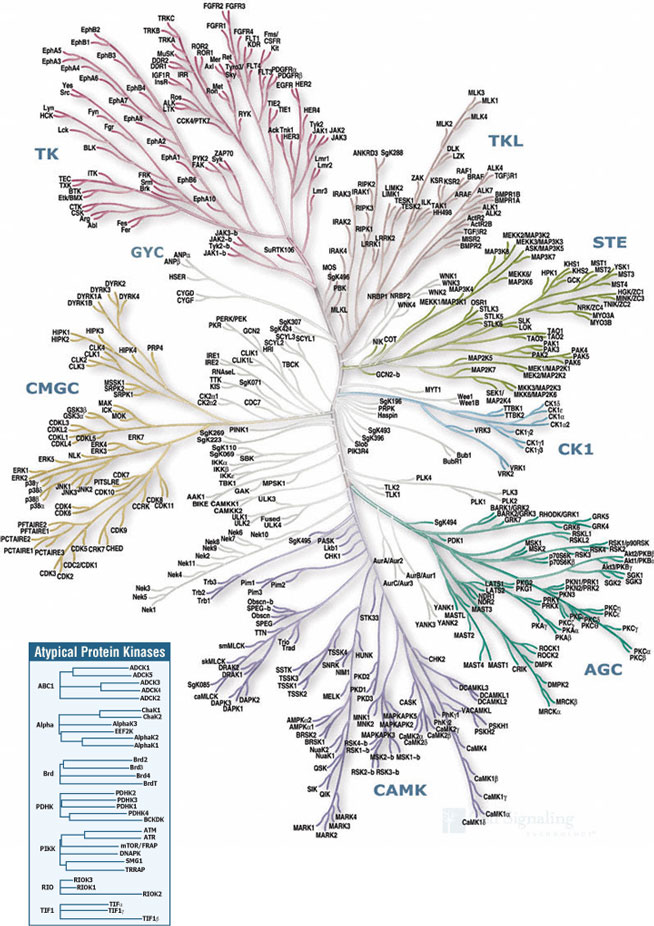
\includegraphics[width=.8\linewidth]{figures/kinome.jpg}
	\centering
	\caption{The human kinome. Kinome illustration courtesy of Cell Signalling 			Technology, Inc (www.cellsignal.com) based on \cite{manning2002protein}.}
	\label{KinomeDendogram}
\end{figure}
\subsection*{Classification of Protein Kinases}
\redcomment{AMG: Just a sentence... I guess you could introduce a bit more the work by Manning before explaining his classification. This introduction could include some evaluation on how his classification holds 15 years later. Also the descriptions of each group below is a bit tedious. I'd suggest you condense it and try to orient the description of each group towards the focus and interest of this chapter i.e. protein kinases as pharmacological targets.}
Below, the groups identified by \cite{manning2002protein} are described in more detail. \\

\textbf{AGC Kinases}\\ 
\redcomment{AMG: this typography is very similar to that of the subsection heading above in the compiled document. It doesn't look like these paragraphs belong to the same subsection}
These group of kinases include PKA, PKG, and PKC. They are involved in diverse cellular roles such as cell growth and proliferation, cell survival, glucose metabolism and protein synthesis. They are also dysregulated in several diseases such as cancer and neurological disorder, inflammation and viral infection \cite {rakshambikai2015typical}. The Akt isoform possesses the pleckstrein homology domain (PH-domain) at the N-terminal and with this domain, it interacts with PIP3 and PIP2  which leads to the activation of pyruvate dehydrogenase kinase isoenzyme (PDK1). PKC also interacts with DAG and calcium by its N-terminal conserved domains (C1 and C2) which leads to conformational changes and activation of the protein \cite{duong2013human}.\\
\begin{figure}[H]
	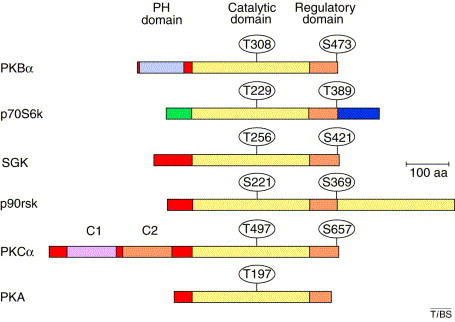
\includegraphics[width=.8\linewidth]{figures/agc_kinase.jpg}
	\centering
	\caption{The domain structure of AGC kinase family. All members contain Thr/Ser in the activation loop. Figure taken from \cite{brazil2001ten} }
	\label{agc_kinase}
\end{figure}
\textbf{CAMK Kinases}\\
These kinases are involved in calcium signalling and are basically autoinhibited. The binding of Ca\textsuperscript{2+}/calmodulin complexes relieves this autoinhibition. Members of this group include MLCK, RAD53, PKD, CAMK2, Trio, CAMKL, DCAMKL, CASK, and DAPK subfamilies and they are all in multidomain architectures. Each member of this family possess additional unique domains in addition to the conserved kinase domain. For instance, the CASK (Ca\textsuperscript{2+} /calmodulin dependent serine kinases) contains a series of L27 repeats, PDZ, two Src homology 3 (SH3) domain as well as a C-terminal guanylate kinase domain \cite{rakshambikai2015typical}. The PKD kinase also possesses a PH domain as found in the Akt family and this is important for the regulation of its enzymatic activity.\\
\begin{figure}[H]
	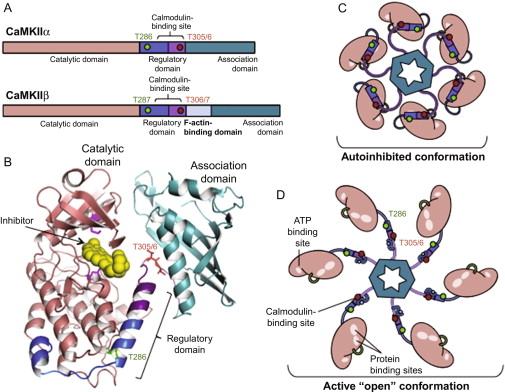
\includegraphics[width=.8\linewidth]{figures/camk_kinase.jpg}
	\centering
	\caption{Domain organisation and structure of CaMKII. (A) Similar domain organisation in the CaMKII$\alpha$ and CaMKII$\beta$ with the exception of F-actin binding domain inserted in CaMKII$\beta$. (B) Structure of autoinhibited CaMKII subunit PDB ID: 3SOA, (C) Cartoon showing the compact inactive holoenzyme (D) Cartoon showing conformational changes associated with CaMKII activation.}
	\label{camk_kinase}
\end{figure}
\textbf{CK1 group}\\
The members of this group are quite ubiquitous in their phosphorylation events as they have a wide range of substrates. They are Ser/Thr kinases and are constitutively expressed. The kinases in this group do not possess additional non-catalytic domains apart from the CK1-gamma subfamily which possesses CK1-gamma domain whose function is not yet known.\\
\begin{figure}[H]
	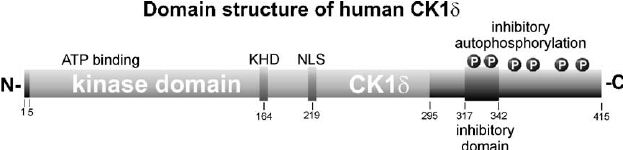
\includegraphics[width=.8\linewidth]{figures/ck.jpg}
	\centering
	\caption{Domain structure of human CK1$\delta$y. The members share a common conserved kinase domain but differs in their variable N-and-C terminal domains. The regulatory c-terminal domain has multiple inhibitory autophosphorylation sites. The nuclear localization signal(NLS) and kinesin homology domain (KHD) are also located within the kinase domain. Figure obtained from \cite{knippschild2005role}}
	\label{camk_kinase}
\end{figure}
\textbf{CMGC group}\\
Members of this group possess single domains like the CK1 group. They include dual specificity tyrosine regulated kinases, dual specificity yak-related kinases(DRYK), cyclin-dependent kinases (CDKs), MAPK, GSK-3, CDK-like kinases. CDKs regulates the progresion through the different phases of the cell cycle in association with their activating partners cyclins. The MAP kinases are amongst the highly studied signal molecules. The MAP kinase cascade include control of proliferation, differentiation, and cell-death across various eukaryotes. The GSK-3 kinases are key metabolic enzyme in glycogen metabolism and play a role in the \textit{Wnt} pathway which is important in embryonic development. \\

\textbf{Tyrosine Kinase group (TK-group)}\\
These kinases catalyse the phosphorylation of tyrosine residues and are heavily implicated in cancer. They are classified into receptor and non-receptor (cytosiolic) kinases. The receptor TKs are classified based on the sequence homology and the structure of their extracellular domains into 20 families. One of the most studied extracellular domain is the Ig-like domain which occurs in most of the members of this subgroup. The extracellular domains acts as the ligand binding sites for several growth receptors. The non-receptor kinases are subdivided into 10 families which include Src, Abl, Ack, Csk, Fak, Fes, Frk/Fyn, Tec and Syk \cite{rakshambikai2015typical}. In addition to the kinase catalytic domain, they also possess additional domains that are important for enzymatic regulation and substrate recognition. Src families for instance possess additional SH3, SH2 domains.The Abl has an F-actin binding site and a DNA-binding region, Fak possess a ferm domain and a focal adhension-binding domain which are important for mediating protein-protein interation \cite{duong2013human,rakshambikai2015typical}.\\
\begin{figure}[H]
\centering
	\begin{subfigure}{\textwidth}
	  \centering
	  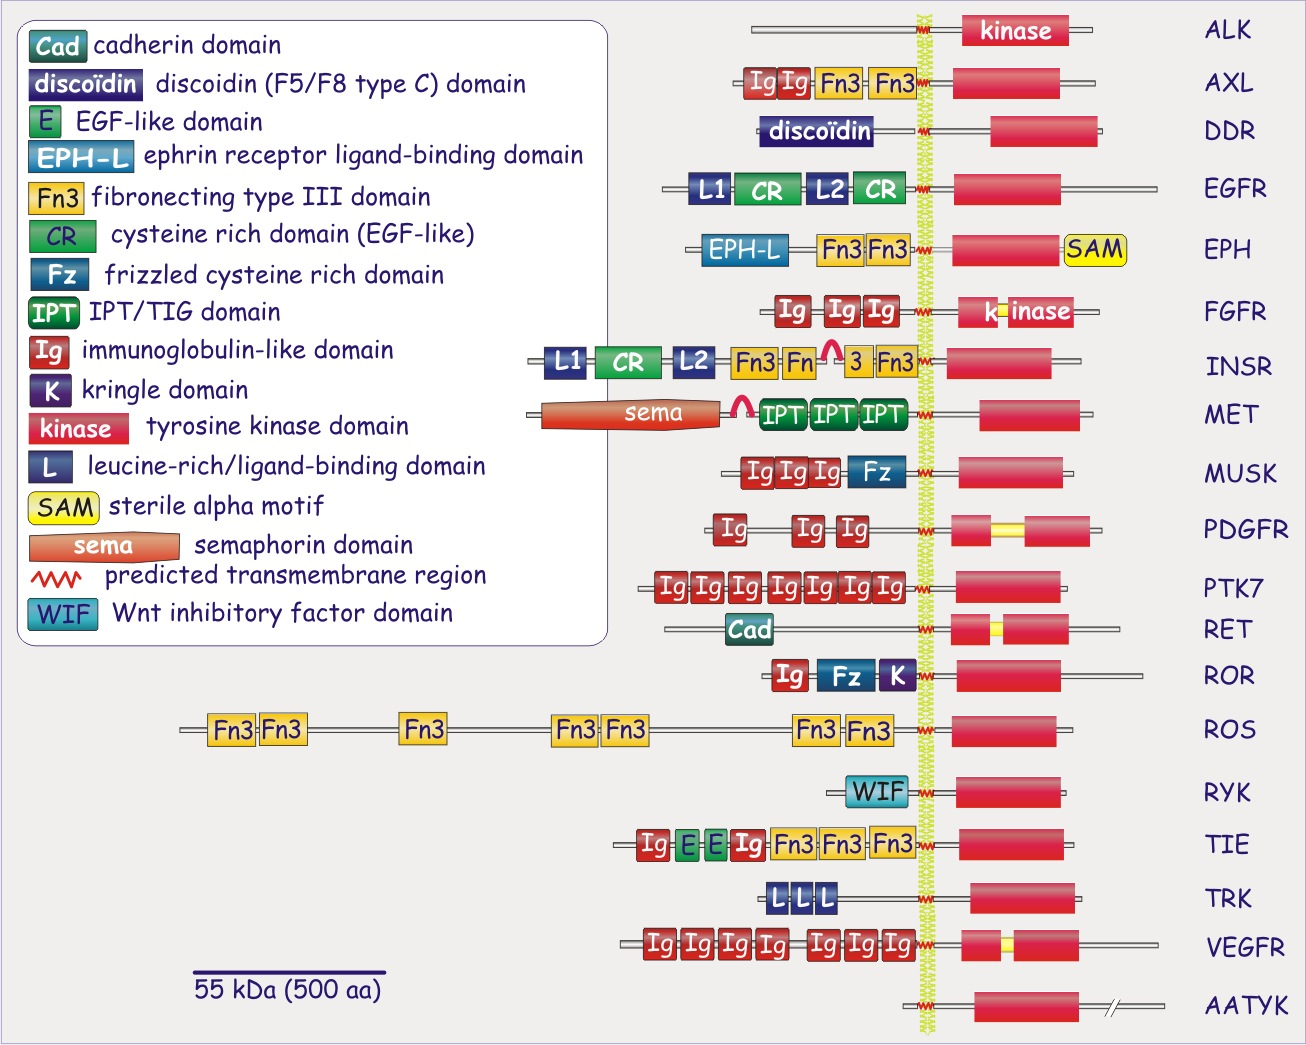
\includegraphics[width=\linewidth]{figures/rtk.jpg}
	  \caption{Receptor protein tyrosine kinase}
	  \label{rtk}
	\end{subfigure}\\
	\begin{subfigure}{\textwidth}
	  \centering
	  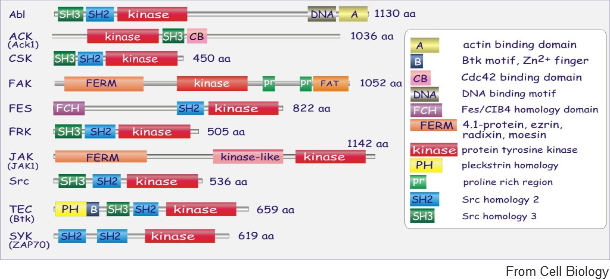
\includegraphics[width=\linewidth]{figures/nrtk.jpg}
	  \caption{Non-receptor protein tyrosine kinase families}
	  \label{nrtk}
	\end{subfigure}
\caption{The multidomain architecture of tyrosine kinases. Figure taken from \cite{foreman2010textbook}. }
\label{tyrosine_kinase}
\end{figure}

\textbf{Tyrosine kinase-like group (TKL group)}\\
The members of this group have close sequence similarity to tyrosine kinases, however, they are mostly serine/threonine kinases and lack the TK-specific motifs. They are mostly diverse with members including receptor and nonreceptor kinases. They comprise of 8 major subfamilies which include IRAK, STKR, RIPK, RAF, LRRK, MLK, MLKL, and LISK.\\

\textbf{STE-group}\\
The members of this group are classified into three major families. They include STE20 (MAPK4), STE11 (MAPK3) and STE7 (MAP2K).  STE stands for "Sterile" and it was originally identified in yeast. The STE kinases sequentially activate each other to then activate the MAPK family.\\

\textbf{RGC-group}\\
The receptor guanylate cyclase represents the smallest group of the kinases and they consist entirely of pesudo-kinases that lack certain residues that are critical for phosphate transfer \cite{manning2002protein}. They convert GTP to GMP\\

\textbf{Others}\\
These include members that lack sufficient sequence similarity to those given above but display unusual phosphorylation properties using ATP and GTP as phosphate donor. Examples include CK2, IKKs.\\

\textbf{Atypical protein kinases (aPks)}\\
The atypical kinases represents group of human kinases that lacks similar sequence identity with the ePKs kinase domain HMM profile but have been shown experimentally to have protein kinase activity. Examples includes PIKK family, A6 family, RIO and Pyruvate dehydrogenase kinase \cite{manning2002protein}.\\ 
\begin{figure}[H]
	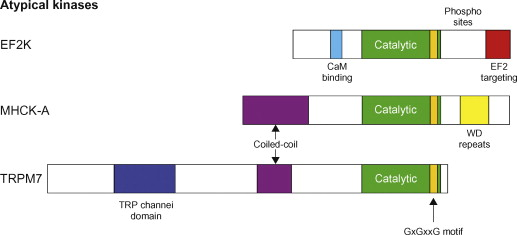
\includegraphics[width=.8\linewidth]{figures/atypical.jpg}
	\centering
	\caption{Domain organisation of atypical family of protein kinases. In contrast to classical kinases, the GXGXXG motif of atypical kinases is not involved in MgATP binding but likely involved in peptide interaction.}
	\label{atypical}
\end{figure}
The crystal structure of the catalytic domain of TRPM7 provides insights into the enzymatic function of the atypical kinases. The comparison of the structure of TRPM7 and PKA catalytic domain reveal some of the major differences between these two. See Figure \ref{atypical2}. 
\begin{figure}[H]
	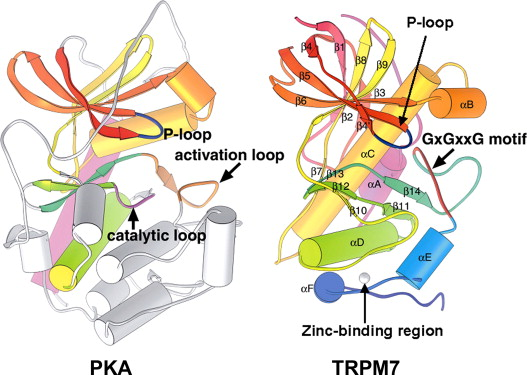
\includegraphics[width=.6\linewidth]{figures/atypical2.jpg}
	\centering
	\caption{Structural comparison of the kinase domains of TRPM7 and PKA. The N-lobe of both PKA and TRPM7 is largely comprised of $\beta$-strands while the MgATP binds at the cleft formed from both the N and C-lobes and the binding of Mg in both also involve the conserved P-loop. However, the catalytic loop is not conserved. The GXGXXG motif in TRPM7 contains an extended loop that may play a similar role as the activation loop in classical protein kinase, PKA. Figure obtained from \cite{wiseman2010ef2k}.} 
	\label{atypical2}
\end{figure}
%\newpage
\subsection*{Structural Features of Protein Kinase}
\redcomment{AMG: Introduce the general (multidomain) structure of protein kinases before going through the description of the kinase domain}
The kinase domain has two dissimilar lobes \redinsert{(the N-lobe and the C-lobe)} joined by a peptide coil called the linker. \redcomment{AMG: The linker is the hinge region below? Now this section is not clearly ordered. I feel the text would gain in clarity if you give a structural overview first (start describing the general structure i.e. lobes and linker/hinge), and after that describe the smaller elements (loops, motifs, binding/functional regions...)} The N-lobe has about 90 amino acids that are orgnised into 5 $\beta$-strands and one helix (C-alpha-helix). This lobe contains the nucleotide binding site that recognises and binds ATP. \redcomment{AMG: I'd provide a brief description of the C-lobe here, and the linker}
In the N-lobe, there are highly conserved sequence motifs that are embedded within the first three stands. The first is the GXGXXG motif (Gly-rich loop) which is between $\beta$1 and $\beta$2. This loop folds over the nucleotide and positions the  $\gamma$-phosphate of the ATP for catalysis. It is the most flexible part of the N-lobe \cite{taylor2011protein}. Another important loop is the P-loop also called the Walker-A motif (GXXGKT/S). Both the glycine rich motif and the P-loop binds to the nucleotide bound phosphate, however, their interaction with the purine is different. For instance, the P-loop does not contact the purine moeity of the ATP while the gly-rich loop connects both $\beta$ strands that at habours the adenine ring; the Gly-rich loop is also followed by a conserved Val within the $\beta$2 strand that makes hydrophobic contact with the base of the ATP \cite{fabbro2015ten}. The third important motif is the AxK motif which is found in the $\beta$3 strand. The lysine from this motif couples the $\alpha$ and $\beta$-phosphate of the ATP to the C-helix. \\
\begin{figure}[H]
	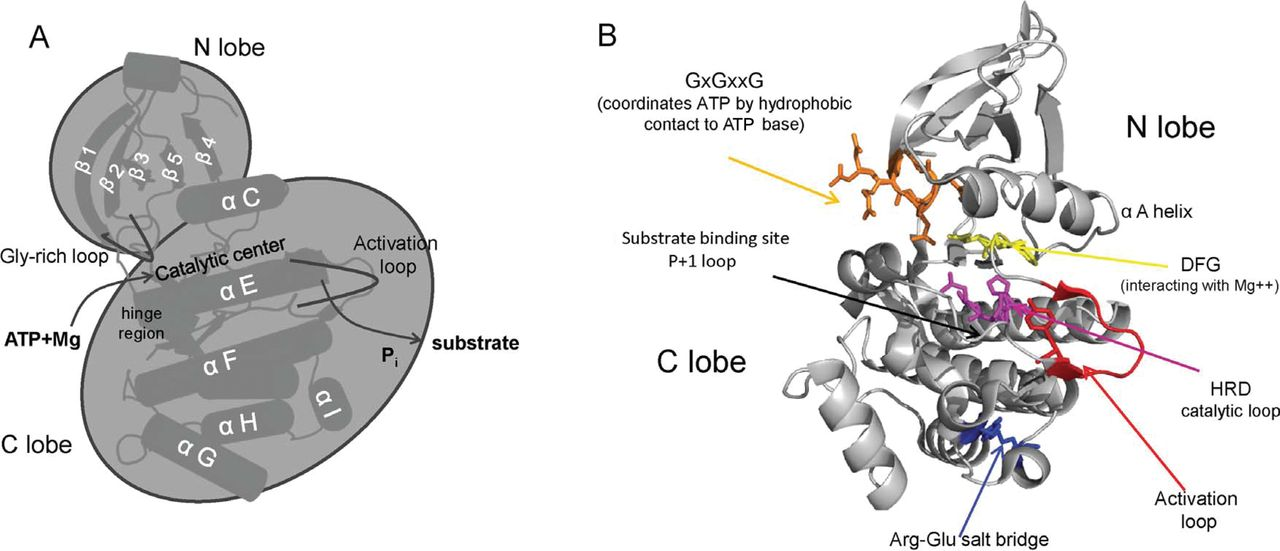
\includegraphics[width=\linewidth]{figures/kinasedom.jpg}
	\centering
	\caption{Schematic overview of kinase features. (a). General overview of the organisation of the kinase domain (b) Conserved motifs and residues of the catalytic core of the protein kinases. Taken from \cite{lorenzen2014hdx}.}
	\label{kinasedoms}
\end{figure}
The C-helix serves as a "signaling integration motif" as it connects to different parts of the kinase domain (See Figure \ref{kinasestructure}a). Its C-terminus is connected to the C-lobe by the $\alpha$C-$\beta$4 loop whereas the N-terminus interfaces with the activation loop. The correct positioning of the C-helix is a step required for the activation of the kinase. The distance between the N-terminus and the activation loop of the C-helix is a measure of the open and closed conformation which is essential for the catalysis \cite{taylor2011protein}. The C-helix is also important in understanding the switch of active to inactive state of protein kinase see section below.\\

The C-lobe however varies in size, sequence and topology. It is predominatly alpha-helical but also contains a few beta strands. It contains the substrate binding groove, activation loop and the catalytic residues. The helical subdomain forms the core of the kinase and the protein/peptide binding surface. The backbone amide of the core helices (D, E, F and H) are well protected from contact with solvent, however, the G-helix is exposed to the solvent. The $\beta$-subdomain comprises 4 short $\beta$ strands (6-9) and contains much of the catalytic machinery for transfering the associated phosphate from the ATP to the protein substrate. The substrate binding site is formed by the hydrophobic residues contributed by the helical core. The activation segment is marked by a conserved DFG (magnesium positioning loop) and APE motif. The activation loop extends from the DFG motif to the Aspartate at the beginning of the F-helix. The length and sequences of the activation segment are the most variable part of the kinase core and this is responsible for turning on and off the kinase \cite{taylor2011protein}. Furthermore, the F-segment extends to the GHI-domain where substrates and regulatory proteins bind. This part is also responsible for stabilizing the active kinase core and also for its allosteric sites (See Figure \ref{kinasestructure}c).\\

The hinge region of the kinase represents the connecting loop between the N and C-lobe. It contains several conserved residues which provide the catalytic machinery and make up part of the ATP binding pocket. The local spatial pattern (LSP) alignment of protein kinase (a method for comparing two protein structures and identifying spatially conserved residues) revealed two hydrophobic motifs called "spines," that connects the N and C-lobe. These spins give insight into how an active protein kinase is assembled differently from an inactive protein kinase \cite{taylor2011protein}. The R-spine comprises four non-consecutive hydrophobic residues; two from the N-lobe (Leu\textsuperscript{106} from $\beta$4 and Leu\textsuperscript{91} from C-helix) and the other two from the C-lobe (Phe\textsuperscript{185} from the activation loop and Tyr\textsuperscript{164}  from the catalytic loop. The R spine is therefore an hydrophobic spine that links the two lobes. Using the LSP on the conserved core of the protein kinase, another hydrophobic spine was identified which is called the catalytic(C)-spine. Like the R-spine, it comprises hydrophobic residues belonging to both lobes. In the N-lobe, the Val\textsuperscript{57} in the $\beta$2 and Ala\textsuperscript{70} from the AxK-motif as well as the Leu\textsuperscript{173} in the C-lobe that docks directly onto the adenine ring of the ATP forming the C-spine. Both spines are anchored to the hydrophobic $\alpha$F-helix . Once the R-spine is assembled, and the C-helix is correctly oriented, then the kinase is primed for catalysis. The binding of ATP completes the C-spine and commits the kinase for catalysis \cite{taylor2011protein,fabbro2015ten,roskoski2016classification}.
\begin{figure}[H]
	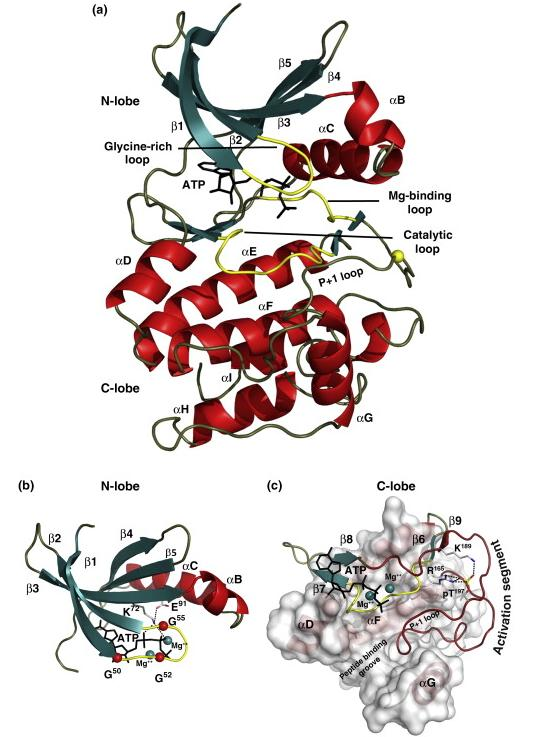
\includegraphics[width=.7\linewidth]{figures/proteinkinase.jpg}
	\centering
	\caption{The structure of conserved kinase core. (a) Protein kinase with the characteristic bilobal. (b) In the N-lobe structure, the glycine rich loop coordinates the ATP phosphate binding while the $\beta$3 strand couples the phosphates and the C-helix. (c) Catalytic and regulatory machinery bound to the rigid core of the C-lobe \cite{taylor2011protein}}
	\label{kinasestructure}
\end{figure}

\subsection*{Active and Inactive Protein Kinases}
\label{sec:kinasereg}
The structure of protein kinases reveals the conformational variation of active and inactive kinases. One of the most common forms of inactive  protein kinases is the assumption of the DFG-Asp of the activation segment in a out-conformation where the aspartate is directed outward whereas the DFG-Phe is directed inward towards the active site \cite{roskoski2016classification}. Structural elements of the kinases show distinct conformation in the active and inactive state. The activation loop for instance is usually in an extended conformation in its active state whereas it is disordered with the loop collapsed to block the substrate binding, in the inactive state (see Figure\ref{kinstruct}). The phosphorylation of the residues within the activation loop activates the kinases \cite{roskoski2016classification}. 
\begin{figure}[H]
	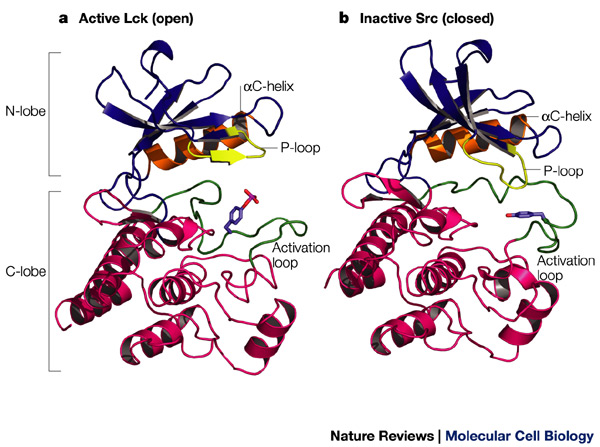
\includegraphics[width=.8\linewidth]{figures/actkin.jpg}
	\centering
	\caption{The active and inactive conformation of LCK and Src respectively. (a) Active conformation with activation loop adopting an extended conformation while it folds in the inactive c-Src kinase domain (b). Figure taken from \cite{hantschel2004regulation}.}
	\label{kinstruct}
\end{figure}
Furthermore, the presence of a salt bridge between the $\beta3$-lysine and the $\alpha$C-glutamate, together with the formation of the R- and C-spine, are the hallmarks of an active kinase domain while inactivation involves the diassembly of the R-spine. The rotation or shift of movement of the $\alpha$C-helix also cause a switch from an inactive to an active kinase as the $\alpha$C adopts an in-conformation in its active state and an out-conformation in its inactive state. \cite{tsai2013molecular,roskoski2016classification}.

\section*{Kinase Inhibitors}
The kinases are quite diverse in their primary sequences. However, they share a great degree of similarity in their 3D structure most especially in their catalytic site where the ATP-binding cavity is found; a $\beta$ sheet containing N-lobe as well as $\alpha$ helix dominated C-terminal (C-lobe) with a connecting hinge region. ATP binds in the cleft between the N and C lobes and therefore most kinase inhibitors interact with this region to perturb the binding of ATP \cite{wu2015fda}. There are several kinds of inhibitors that are being exploited in targeting protein kinases. These inhibitors differ in their mode of binding and the mechanism of action exhibited upon binding. The kinase inhibitors can either bind covalently or reversibly.\\
The nonreversible (covalent) inhibitors bind irreversibly with the reactive nucleophilic cysteine or lysine residue close to the ATP-binding site resulting in the blockage of ATP binding and leading to irreversible inhibition. Example of such a drug in clinical trial is the AVL-292 which is a tyrosine kinase inhibitor which covalently binds to the Bruton tyrosine kinase (BTK)\cite{robak2012tyrosine}, ibrutinib targets BTK as well, while afatinib targets the gefitinib resistant EGFR \cite{akinleye2014ibrutinib}.\\
\begin{figure}[H]
	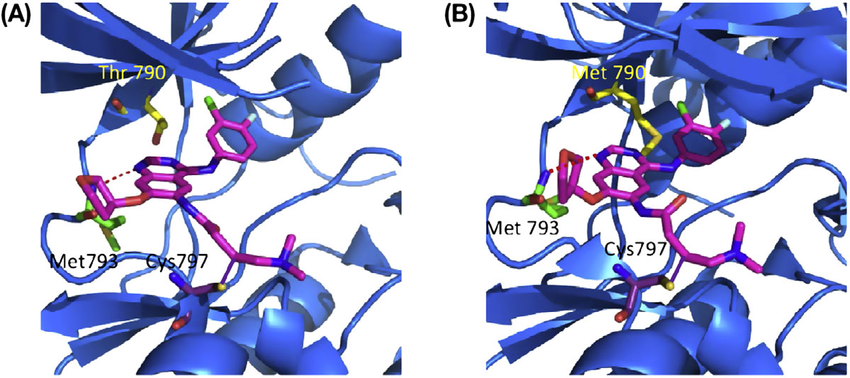
\includegraphics[width=.8\linewidth]{figures/Afatinib.jpg}
	\centering
	\caption{Afatinib co-crystal structure with wild-type EGFR (PDB ID: 4G5J) and mutant T790M EGFR (PDB ID:4G5P). Afatinib binds to the kinase domain in its active conformation and forms a hydrogen bond with the backbone NH of Met793 and also forms covalent interaction with the sulphur of Cys797. Figure obtained from \cite{hossam2016covalent}}
	\label{afatinib}
\end{figure}
The reversible (non-covalent) inhibitors on the other hand can be classified into several types, based on their interaction with binding pocket and the DFG motif (hinge region). The type-1 inhibitors are ATP-competitors that bind to the active form of the enzyme with the aspartate residue of the DFG motif facing the active site of the kinase (DFG-in conformation). The conserved Phe of the DFG-motif is buried within the hydrophobic pocket of the groove between the N and C-lobes. Most of the compounds that target this active conformation have been selected using enzymatic assays that select ATP mimetics with the highest inhibitory activity for the kinase \cite{fabbro2015ten}. Classical examples of such approved inhibitors include gefitinib, dasatinib, erlotinib and sunitinib.\\ 
\begin{figure}[H]
	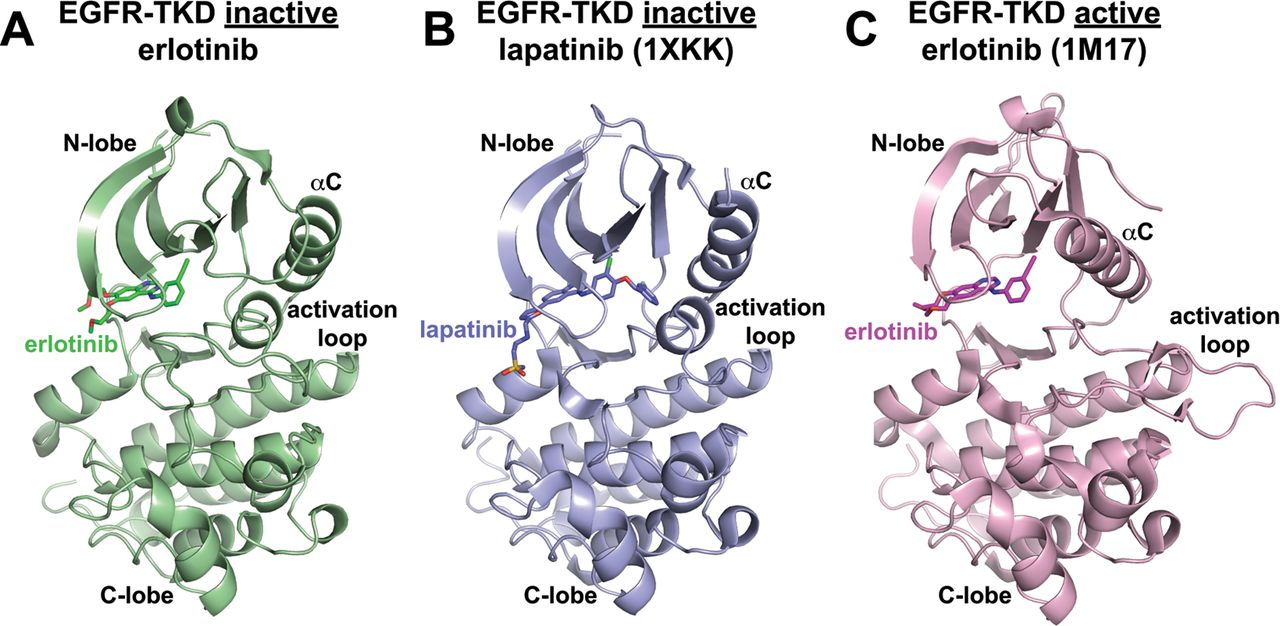
\includegraphics[width=.8\linewidth]{figures/erlotinib.jpg}
	\centering
	\caption{Crystal structure of EGFR tyrosine kinase domain (TKD) bound with inhibitors. (A)Erlotinib  bound with EGFR-TKD in the inactive state (B) Lapatinib with inactive EGFR-TKD (1XKK) (C) Erlotinib with the active EGFR-TKD (1M17). Figure obtained from \cite{park2012erlotinib}}
	\label{erlotinib}
\end{figure}
The type-2 inhibitor binds to the inactive form of the enzyme with the aspartate residue of the DFG motif protruding outward from the ATP-binding site of the kinase. The transition from the DFG-in to DFG-out conformation exposes the hydrophobic pocket adjacent to the ATP-binding site and this is utilized by the type-2 inhibitor to lock the kinase in an inactive conformation \cite{cowan2009structural}. The type-2 are generally less promiscuous as compared to the type-1 inhibitors. Examples of FDA-approved type II kinase inhibitors include imatinib, nilotinib, and sorafenib \cite{fabbro2015ten}. The type-1 and 2 inhibitors however face competition with the millimolar concentration of ATP \textit{in vivo} as well as lack of selectivity due to the extensive adenosine binding cleft \cite{lamba2012new}. There have therefore been  efforts directed towards kinase inhibitors with high selectivity, high affinity and less side effects from usage.\\
The type-3 inhibitors are a heterogeneous group of kinase inhibitors that bind to allosteric or remote sites on the kinase. These inhibitors mostly do not bind at the ATP-binding sites and have no physical contact with the hinge and they have been shown to exhibit the highest form of selectivity by exploiting the binding and regulatory sites that are specific to a particular kinase \cite{fabbro2015ten}. The combinations of the structural elements in the kinases such as the C-helix's DFG-in and out state, A-loop, G-loop, C-terminal elements as well as regulatory domains can be exploited to design selective inhibitors with clear advantage over the type-1 and 2 inhibitors \cite{cowan2009structural}. Examples of approved type-3 inhibitors include cobimetinib, trametinib, selumetinib, binimetinib and rapamycin. Type-3 inhibitor of MEK1 binds to the adjacent pocket to the ATP-site which is referred to as the "allosteric back pocket-DFG-in" in the presence of ATP and "allosteric back pocket-DFG-out" in the absence of ATP \cite{fabbro2015ten}. 
\begin{figure}[H]
	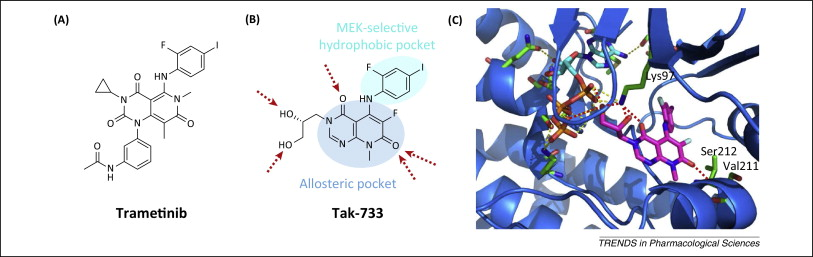
\includegraphics[width=\linewidth]{figures/trametinib.jpg}
	\centering
	\caption{MEK kinase inibitor binding mode (A). The chemical structure of trametinib (B) The binding mode of trametinib with MEK1 (C). Tak-733 co-crystallized with MEK1 (PDB ID: 3PPI) ATP is shown in cyan and Tak-733 in magenta. Figure taken from \cite{wu2015fda}}.
	\label{trametinib}
\end{figure}
The type-4 allosteric inhibitors bind at allosteric sites that is distant from the ATP-binding site. A unique example is the AktI-1/2 targeted inhibitor that inhibits Akt isoforms 1 and 2 kinases. Interestingly, \redcomment{AMG: why is this interesting? Check out for unnecesary adverbs throughout the text} 
 these inhibitors \sout{has no inhibition} \redinsert{have no effect} against PH-domain mutants which suggest that the PH domain is required to exert their activity. This clearly shows that the inhibitor interacts with both the catalytic domain and the PH domain and prevents the activation of the upstream kinase PDK1 \cite{barnett2005identification}. Other types of allosteric protein kinase inhibitors includes the type-5 which are also referred to as bivalent or bi-substrate inhibitor. The bivalent inhibitors tend to have high affinity and more selectivity for targeted therapy. The design of such inhibitors involve the use of an appropriate linker to couple allosteric site inhibitor with kinase active site binding agent to achieve improved selectivity from the non-ATP directed inhibitor \cite {lamba2012new}. Other examples of kinase inhibitors is the hybrid-type having both type I and II features. The field of allosteric kinase inhibition is a rapidly evolving field with the FDA-approval of trametinib as well as several other allosteric inhibitors that are in clinical trials \cite{wu2015allosteric}.
\begin{figure}[H]
	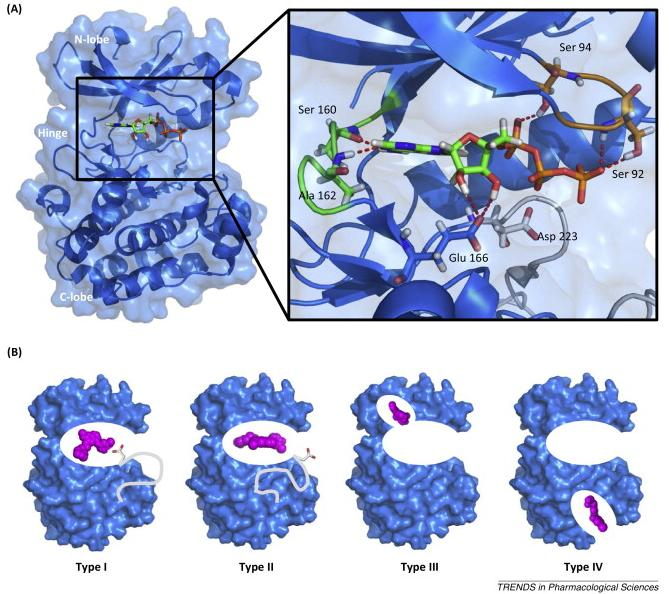
\includegraphics[width=.8\linewidth]{figures/kinase_inhibitors.jpg}
	\centering
	\caption{Kinase structure and the various types of inhibitor schematics. (A). Co-crystal structure of PDK1 with ATP (adenine and ribose in green, phosphate in orange) Enlarged area shows hydrogen bond in red, hinge and hinge residues in green backbone, P-loop and P-loop residues in brown-orange, Asp residue of the DFG motif  and the activation loop in grey [PDB ID:4RRV, 1.41A], (B) The four types of reversible binding  mode. Figure taken from \cite{wu2015fda}}.
	\label{type4inhibitor}
\end{figure}
Allosteric inhibition offer some advantages such as high  selectivity and ability to overcome drug resistance as most drug resistance to small molecule kinase inhibitors occurs frequently around the hinge region. However, some debated opinion about allosteric inhibitors include; mutation-related resistance may occur at the allosteric sites as they are not as essential for kinase function as the ATP binding sites. Also, as a result of the hydrophobic properties of most allosteric pockets, the allosteric inhibitors are lipophilic compounds and this may result in poor bioavailability, and poor solubility. Another major challenge is the limited numbers of structures for allosteric-inhibitor-bound kinases to help in the comparison of the induced changes associated with the on/off-bound state of the enzymes. This may be due to the fact that these sites are involved in protein-protein and protein-peptide interactions and the transient nature of such interactions creates difficulty in solving the structures. \cite{wu2015allosteric}.

\subsection*{Understanding the promiscuity of Protein Kinase Inhibitors}

Protein kinase inhibitors are generally considered promiscous because of their lack of specificity and ability to interact with several kinases and families, due to the presence of the conserved ATP-binding site where the kinase inhibitors interact with. Promiscuity is defined as the ability of a compound to specifically interact with more than one target (the target of interest for which it was designed \cite{hu2017mapping}. Hu et al classified the protein kinse inhibitors into single and multiple kinase inhibitors based on the numbers of targets the PKI compounds in ChEMBL database were active against. Furthermore, they also assessed the promiscuity of a kinase for several structurally diverse compounds and found that many kinases recognises structurally diversed compounds \cite{hu2017mapping}.\\

\redcomment{AMG: You need to comment on the relationship between promiscuity and safety}

In the work earlier reported by \cite{zhang2008turning}, they understood this concept of cross reactivity and promiscuity associated with kinase inhibitors. However, they identify some "selective filters" can may be used to distinguish safer drugs and targets from the list of paralog targets the drugs might be associated with. This selective filters are called dehydrons which are also referred to as "wrapping patterns" of the protein targets. They are the intermolecular protection of backbone hydrogen bonds from the hyration of amide and carbonyl groups. The wrapping defects could be informed not only from the structure of the protein kinase but also the sequence. The incorporation of dehydrons into drugs designs have been shown to reduce the numbers of cross-reactivity and improve the specificity of protein kinase inhibitors \cite{zhang2008turning}.
\newpage
\section*{Objectives}
We have previously demonstrated the importance of using CATH-FunFams as a reasonable annotation level for drug-domain interaction and also used network analysis to associate the propensity of side effects with the network properties of these families through our druggable FunFam approach \cite{moya2017structural}. In this study, we are focusing on protein kinase inhibitors, a set of molecules that inhibit the activities of kinases. Using a set of publicly available protein kinase inhibitors, we intend to associate the targeted kinases with our domain-families (FunFams) and subsequently measure some network characteristics to distinguish FunFams with side effects from others. We will also be exploring some similarity measures and structural coherence to shed more lights on possible repurposing of protein kinase inhibitors to members of a given FunFam.
\redcomment{AMG: State that we want to investigate the causes of PKI promiscuity beyond the similarity of ATP/drug binding sites}

\section*{Results and Discussion}
\subsection*{GSK-Protein Kinase Inhibitor\redinsert{s set/data}}
The Published Kinase Inhibitor Set (PKIS) is a collection of 367 compounds that have been made available by GSK to the external community \cite{dranchak2013profile, knapp2013public}. These compounds have been annotated with protein kinase  activity \cite{knapp2013public}. These compounds are of various chemotypes and they are openly available from the ChEMBL database (ChEMBL release 23) \cite{gaulton2016chembl}. The PKIS are active against some known target kinases and can be extended to other new target kinases. We collected only a subset of the PKIS that indicate an inhibitory activity level above 50\% as \cite{dranchak2013profile,  anastassiadis2011comprehensive} had reported this threshold as appropriate for considering the inhibition of kinase catalytic activity. This gave a unique set of 205 protein kinase inhibitors that were distributed across 133 protein kinases. This covers about 60\% of the entire PKIS set and thus a reasonable dataset to consider for a network assessment and characterization of protein kinase inhibition.

\subsection*{Target Promiscuity of Protein Kinase Inhibitors}
The PKIS dataset obtained from ChEMBL database was analysed to study the association of kinases (targets) with inhibitors in order to understand the inherent promiscuity associated with the protein kinase inhibitors set. 

\begin{figure}[H]
\centering
\begin{subfigure}{.6\textwidth}
  \centering
  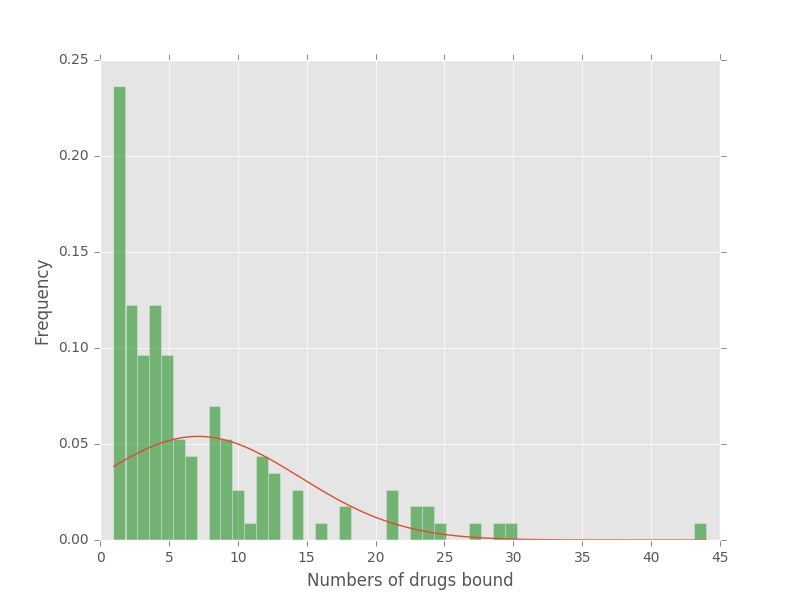
\includegraphics[width=\linewidth]{figures/numb_drugs.png}
  \caption{Promiscuity of drugs for kinases}
  \label{targ_drugdis}
\end{subfigure}%
\begin{subfigure}{.6\textwidth}
  \centering
  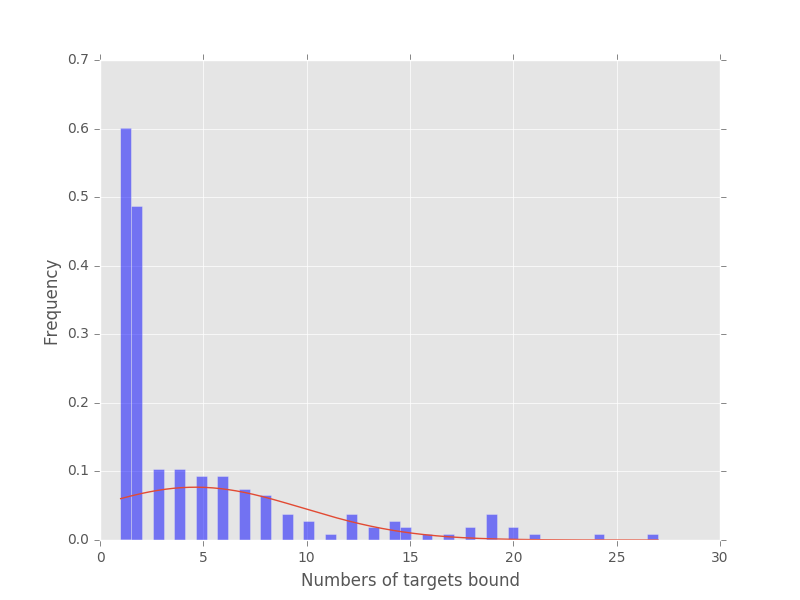
\includegraphics[width=\linewidth]{figures/num_target.png}
    \caption{Promiscuity of targets for PKIS}
  \label{drugtarg}
\end{subfigure}
\caption{Distribution of kinase-drug interaction and drug-kinase interaction for the GSK-PKIS sets}
\label{targ_dis}
\end{figure}
Figure \ref{targ_dis} shows the promiscuity of the kinases for inhibitors as well as inhibitors for kinases. Protein kinase inhibitors interact with more than one kinase  while some kinases could also interact with more than one protein kinase inhibitor, which indicates the non-specificity of these kinase sets.

\subsection*{Mapping kinases to Pfam-FunFam}
Protein kinases have been divided divided into 9 groups by \cite{manning2002protein} as explained in the introductory section. We associated all human kinases with our functional families (groups of evolutionarily related, structurally and functionally coherent protein families). We scanned all human kinase sequences from Pfam against Pfam-FunFams library using HMMer3. Pfam-FunFam data from the Gene3D database was used as Pfam provides sequences that cover the entire kinase catalytic region, whilst CATH divides the kinases into the N and C lobe domains.\\
1277 human protein kinases sequences obtained from Pfam was clustered at 90\% sequence identity to obtain a unique non-redundant human kinase set using CD-HIT clustering algorithm. The 741 unique kinases obtained were distributed amongst 130 Pfam-FunFams. The identified Pfam-FunFam represents 46\% of the entire Pfam-clan as the human protein kinases were associated with 16 of the 35 Pfam clans. We mapped the Pfam-FunFam to the human kinome tree and found that the our domain-family classification are well annotated to the various groups with no overlap between the already identified grouping by \cite{manning2002protein} as shown in figure \ref{kinasetree} below. \redcomment{AMG: the difference between 1227 and 741 proteins merits a brief comment on isoforms and how we deal with them}
\begin{figure}[H]
	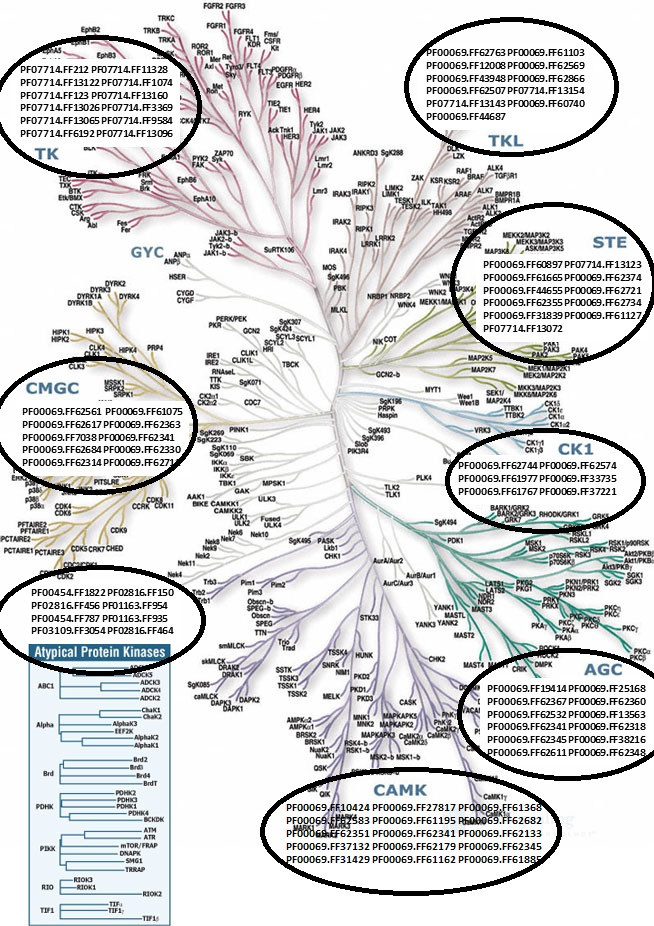
\includegraphics[width=.9\linewidth]{figures/kinometree.jpg}
	\centering
	\caption{Pfam-FunFam distribution across the human kinome.The kinome tree was adapted from \cite{manning2002protein}. The mapping of Pfam-FunFam to the group "Others" is not shown in this figure}
	\label{kinasetree}
\end{figure}
We then mapped the drug-targets of the PKIS obtained from ChEMBL to the Pfam-FunFams at 50\% inhibition level with an affinity of 0.1$\mu$M and found that they are associated with 37 of the 130 Pfam-FunFams which represents about 30\% of the human kinase Pfam-FunFam obtained. We speculated that this 30\% represents the kinases most targeted by the pharmaceutical industry based on their relevance to human disease and those most studied as the current research in kinase therapeutics indicate that only 10-15\% is being targeted, we also observed this ratio from the entire GSK-PKIS set being used in this study.

\redcomment{AMG: this speculation can be easily checked by looking at the functions of these kinases. Also, this kind of shows the upper limit of the real associations between FFs and drugs (not all these associations will be statistically significant and hence we won't consider all of them true associations)}

\subsection*{Conservation of human kinase relatives in the Pfam-FunFams}
We measured how conserved the kinases across the Pfam-FunFam are. The human relatives of the Pfam-FunFam were mapped to structure by SIFT-ing through UniProt sequences to PDB while the domain region were specified using Pfam. The structures were therefore evaluated for structural conservation by measuring RMSD using the SSAP algorithm. The groups were divided into the tyrosine-kinase Pfam-FunFam and serine/threonine Pfam-FunFams. The distribution of the RMSD across the two Pfam-FunFam groups is shown in figure \ref{ssap_measure} below.
\begin{figure}[H]
\centering
\begin{subfigure}{.8\textwidth}
  \centering
  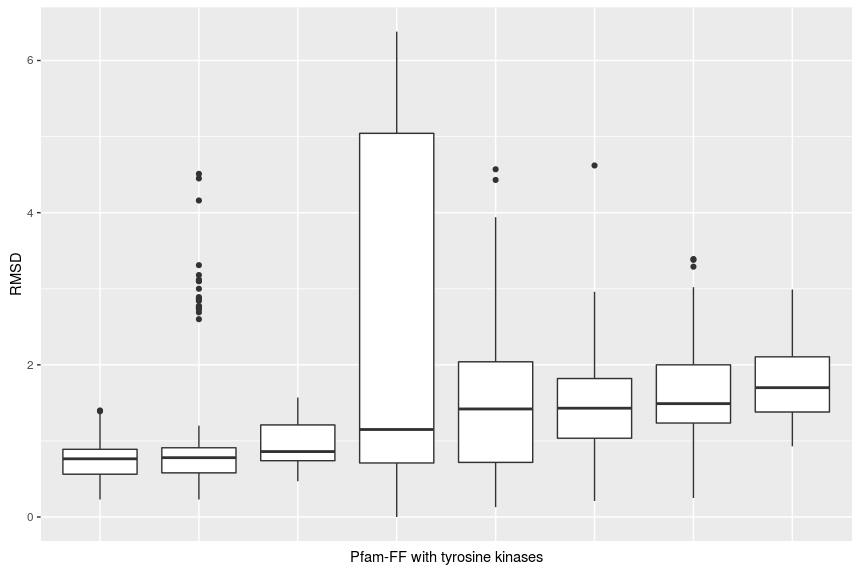
\includegraphics[width=\linewidth]{figures/ssap_tyr.png}
  \caption{RMSD across the Tyr Pfam-FunFam}
  \label{ssap_tyr}
\end{subfigure}\\
\begin{subfigure}{.8\textwidth}
  \centering
  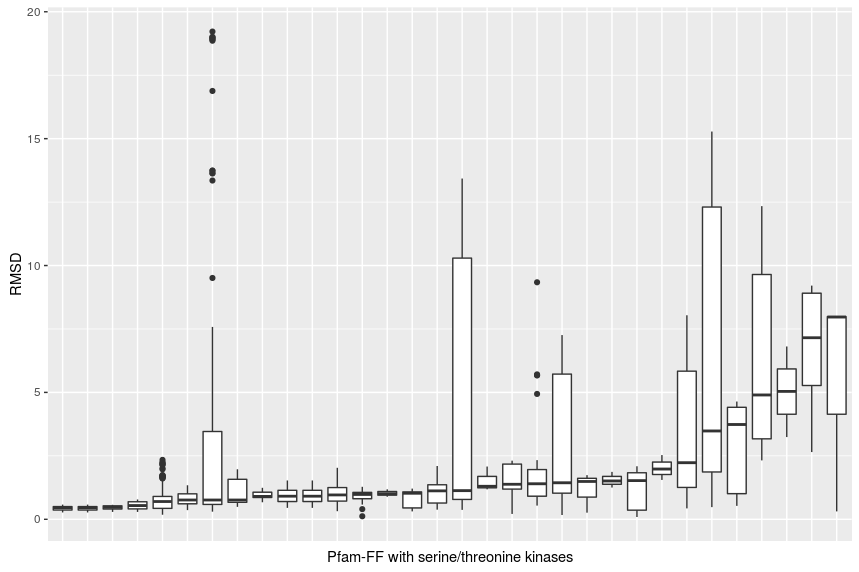
\includegraphics[width=\linewidth]{figures/ssap_ser.png}
    \caption{RMSD across the Ser/Thr Pfam-FunFam}
  \label{ssap_ser}
\end{subfigure}
\caption{Structural coherence and conservation of the Pfam-FunFam kinases measured using the SSAP-algorithm}
\label{ssap_measure}
\end{figure}
The figure \ref{ssap_measure} shows the conservation of the relatives in these families as the observed RMSD was relatively below 2 in both the tyrosine kinases as well as the serine/threonine kinase FunFams. This therefore agrees with the overall view of the structural conservation of the kinases. However, some families show that Pfam-FunFams with members having high RMSD score which tend to distort the overall RMSD measure and indicating lack of structural coherence with relatives of the FunFams.\\
A deeper insight into one of such families was carried out using the Pfam-FunFam PF07714.FF13122 which gave an overall RMSD below 2A but contains outliers that influence some members having RMSD as high as 5A in comparison to other members with low RMSD. The reason for this could be attributed to the multidomain architecture of the relatives of the Pfam-FunFam as majority of the relative in this protein have additional SH2-domain  while others either have an immunoglobulin-domains or no additional domain.


\subsection*{Enrichment test of Pfam-FunFams associated with drug targets}
\cite{anastassiadis2011comprehensive} reported the thorough characterization of the Published Kinase Inhibitor Sets (PKIS) and identified them as the chemical starting point for probing orphan kinases. They illustrated the utility of these compounds for developing selective inhibitors against untargeted kinases LOK and SLK. Thus, the use of domain families could help increase the coverage of potential targets of the kinase-inhibitor set as the targeted kinases are about 10-15\% . We used our enriched FunFam program (see chapter two) to test for the overrepresentation of drugs in our FunFams. This involves using a binomial test followed by multiple testing for correction to determine the most appropriate FunFam with which a Kinase inhibitor associates. We found that PKIS-drugtargets were overrepresented in 30 Pfam-FunFam at p-value $\leq$ 0.05. 109 PKIS were found to be associated with the 30 Pfam-FunFams. \\
\begin{figure}[H]
	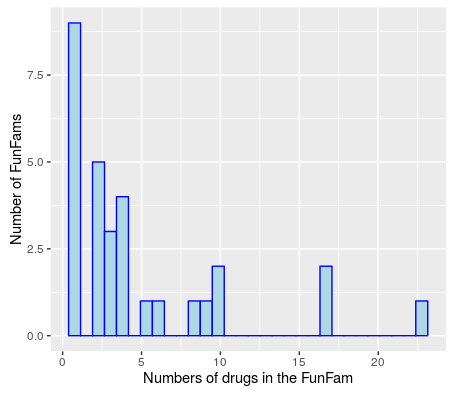
\includegraphics[width=.8\linewidth]{figures/ffdrugdis.png}
	\centering
	\caption{Distribution of drugs in the overrepresented FunFams}
	\label{distdrugFF}
\end{figure}
As shown in figure \ref{distdrugFF}, we observed that 70\% of the enriched Pfam-FunFams were associated with more than 2 kinase inhibitors from the PKIS set. This enriched Pfam-FunFam dataset was used for further analysis of the protein-kinase inhibitor targets on protein-protein interaction network.\\
The Pfam-FunFam-drug interaction was represented in network for visualization in Cytoscape as shown in figure \ref{pfam-chembl} while the names of the overrepresented Pfam-FunFams were identify using our in-house program for the UniProt description  of protein sequences as shown in table \ref{pfam-drug}.
\begin{figure}[H]
	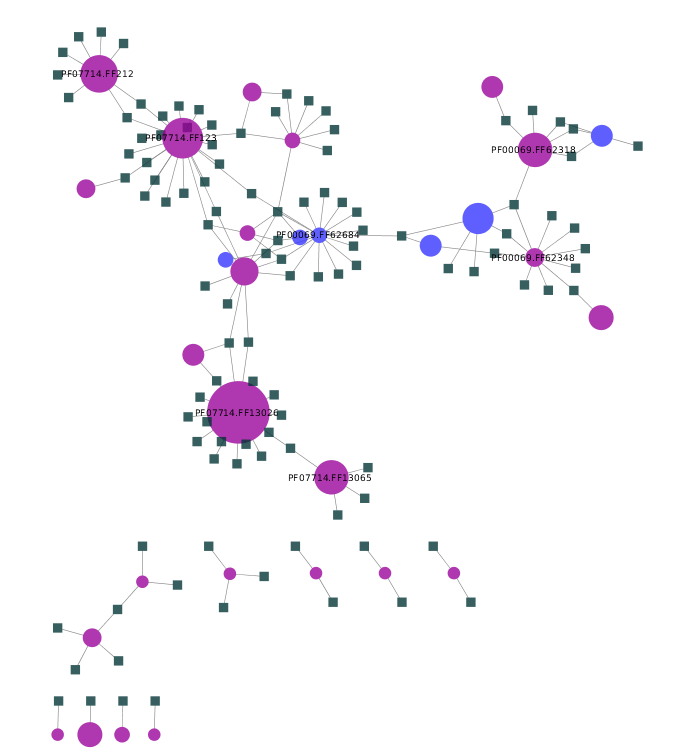
\includegraphics[width=.9\linewidth]{figures/pfam_chembl.png}
	\centering
	\caption{Pfam-FumFam-drug interaction network. In this network, the green coloured square node represents the CheMBL protein kinase inhibitors while the purple coloured circle nodes are the Pfam-FunFam whose relative are quite coherent with a mean RMSD$\leq$ 2 while the blue coloured circle are Pfam-FunFam with RMSD value $\geq$ 2.5. The size of each node reflects the numbers of targets (relatives)\redcomment{AMG: Only known drug targets or all relatives? If all relatives, this meas there is room to find new potential targets for the PKI associated with the FFs} in each family. Also labelled are some interesting families with relatives  $\geq$ 5 and interacting with at least 5 drugs.}
	\label{pfam-chembl}
\end{figure}


\begin{table}[H]
\fontsize{9}{10}\selectfont
\centering
\caption{The overrepresented FunFams and the number of drugs associated with each FunFam.}
\label{pfam-drug}
\begin{tabular}{|c|c|c|}
\hline
Pfam-FunFam    & Uniprot-Description                                                       & No of Drugs \\ \hline
PF00069.FF13563 & Ribosomal protein S6 kinase alpha-5                            & 3            \\ \hline
PF00069.FF25168 & Protein kinase B beta                                          & 4            \\ \hline
PF00069.FF31429 & MAP/microtubule affinity-regulating kinase 3                   & 1            \\ \hline
PF00069.FF31839 & Serine/threonine-protein kinase 4                              & 2            \\ \hline
PF00069.FF37132 & Serine/threonine-protein kinase BRSK2                          & 1            \\ \hline
PF00069.FF62179 & Serine/threonine-protein kinase pim-1                          & 1            \\ \hline
PF00069.FF62314 & Mitogen-activated protein (MAP) kinase                         & 4            \\ \hline
PF00069.FF62318 & p90 ribosomal S6 kinase                                        & 6            \\ \hline
PF00069.FF62341 & Cell division protein kinase                                   & 4            \\ \hline
PF00069.FF62345 & Calcium/calmodulin-dependent serine/threonine-protein kinase 1 & 5            \\ \hline
PF00069.FF62348 & Microtubule-associated serine/threonine-protein kinase 2       & 10           \\ \hline
PF00069.FF62351 & CBL-interacting serine/threonine-protein kinase 1              & 1            \\ \hline
PF00069.FF62355 & Non-specific serine/threonine protein kinase                   & 1            \\ \hline
PF00069.FF62363 & Dual specificity tyrosine-phosphorylation-regulated kinase     & 10           \\ \hline
PF00069.FF62561 & Cyclin-dependent kinase 6                                      & 1            \\ \hline
PF00069.FF62583 & Testis-specific serine/threonine-protein kinase 1              & 2            \\ \hline
PF00069.FF62585 & Serine/threonine-protein kinase Nek8, related                  & 3            \\ \hline
PF00069.FF62682 & MAP kinase-interacting serine/threonine-protein kinase         & 1            \\ \hline
PF00069.FF62684 & Glycogen synthase kinase 3                                     & 17           \\ \hline
PF00069.FF62706 & Ttk family protein kinase                                      & 2            \\ \hline
PF00069.FF62744 & Casein kinase I alpha                                          & 3            \\ \hline
PF00069.FF62866 & Leucine-rich repeat serine/threonine-protein kinase            & 2            \\ \hline
PF00069.FF7038  & Cyclin-dependent kinase 2                                      & 8            \\ \hline
PF07714.FF123   & Platelet-derived growth factor receptor alpha                  & 23           \\ \hline
PF07714.FF13026 & Receptor protein-tyrosine kinase                               & 17           \\ \hline
PF07714.FF13065 & Receptor protein-tyrosine kinase                               & 4            \\ \hline
PF07714.FF13096 & Tyrosine-protein kinase                                        & 1            \\ \hline
PF07714.FF13122 & Non-specific protein-tyrosine kinase                           & 1            \\ \hline
PF07714.FF13154 & LIM domain kinase 2                                            & 2            \\ \hline
\end{tabular}
\end{table}

\redcomment{AMG: Maybe check for the promiscuity within a FunFam (i.e. promiscuity of PKI among the relatives of a FF) for those FF that are/seem to be very important in cancer? This would provide us with interesting material for discussion}

\subsection*{Network Analysis of the Pfam-FunFams Enriched with Drug Targets}
The representation of proteins on a network gives a view of the information flow and interactors for biological process. We obtained a functional protein assocaiation network for human from the STRING database version 10.0. We filtered this data and only used those edges with a combined and database score of $\geq$ 800 which correspond to those PPI with high reliabilty. This gave 219,608 physical interactions between 10,430 proteins. We extracted the largest connected subgraph and then computed the node centralities for drug targets from the enriched Pfam-FunFams using centrality measures such as the betweenness centrality and PageRank. 
\subsubsection*{Centrality Measure}
Centrality measures identify important nodes relative to other nodes within the network. Such measures include the degree, betweenness centrality as well as the PageRank. The degree of a node is the number of connections (edges) it shares with other nodes. The betweenness centrality (BC) is however the fraction of the number of shortest paths that pass through each node. The BC measures how often a node occurs on all the shortest paths between two nodes. Therefore, a node with high BC influences the flow of information in the network. \[c_B(v) =\sum_{s,t \in V} \frac{\sigma(s, t|v)}{\sigma(s, t)}\]\\
\textit{where $V$ is the set of nodes, $\sigma(s, t)$ is the number of shortest (s, t)-paths, and $\sigma(s, t|v)$ is the number of those paths passing through some node v other than s, t. If s = t, $\sigma(s, t) = 1$, and if v $\in {s, t}$, $\sigma(s, t|v) = 0$}\\
We measured the topological properties of the targeted kinases and compared them to all human kinase and all proteins in a given human functional network. we defined here "Hubs" as the top 20\% nodes with highest degree (connections) while "High-BC" are those top 20\% nodes with the highest betweenness centrality. The "Bottlenecks" we have defined as those nodes within the "High-BC" but excluded from "Hubs" i.e. those with low degree connectivity. The "Hubs \& High-BC" are those set of nodes in the Hubs group with high betweenness centrality measure. 
\begin{table}[H]
\centering
\caption{Topological analysis of kinases in a functional protein network}
\label{hubs-bottlenecks}
\begin{tabular}{|c|c|c|c|c|}
\hline
\textit{Groups}             & \textit{Hubs (\%)} & \textit{Bottlenecks (\%)} & \textit{High-BC (\%)} & \textit{Hubs \& High-BC (\%)} \\ \hline
\textit{Targeted Kinases}   & \textit{22.64}     & \textit{2.8}              & \textit{21.69}        & \textit{24.52}                \\ \hline
\textit{All-human kinases}  & \textit{8.08}      & \textit{2.15}             & \textit{7.14}         & \textit{9.3}                  \\ \hline
\textit{All-human proteins} & \textit{19.68}     & \textit{11.56}            & \textit{8.12}         & \textit{19.68}                \\ \hline
\end{tabular}
\end{table}
The measure of degree and betweenness centrality are some of the most profound topological properties of nodes in a protein interaction network. The bottlenecks in a protein functional network represents key connectors and surprisingly show functional and dynamic properties \cite{yu2007importance}. The \redinsert{Table \ref{hubs-bottlenecks} shows the comparison of the targeted kinases, all human kinases and all human proteins in a functional network}. The proportion is a measured relative to each group as; 
\[
\frac{\text{Number of Hubs or bottlenecks in targeted set} \times100 } {\text{Total number proteins in targeted set}}
\]
The result therefore shows that only a small percentage of the targeted kinases are bottlenecks. Our observation shows that on average, the betweenness centrality is lower in the targeted kinases compared to all the proteins in the network, however, the violin oplot in figure \ref{bottle_measured} indicates that some of the targeted kinase have a higher betweenness centrality measure. We hypothesize that bottlenecks will be a good drug target as they are central in the network but associated with less nodes (thus less functional disintegration expected). However, there is still a lot of debate on this opinion as some studies have suggested bottlenecks to be associated with side effects. \redcomment{Discuss this further using this Csermely paper 1.	Perez-Lopez, Á. R. et al. Targets of drugs are generally, and targets of drugs having side effects are specifically good spreaders of human interactome perturbations. Sci Rep 1–9 (2015). doi:10.1038/srep10182}

\begin{figure}[H]
	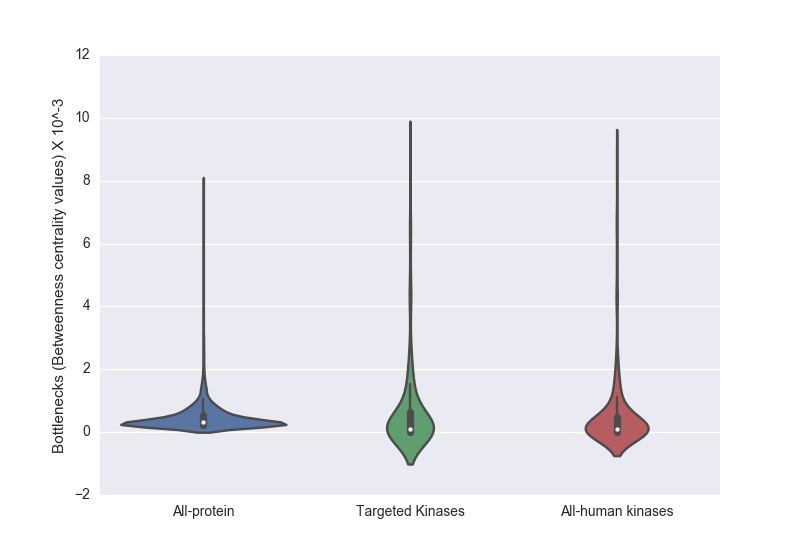
\includegraphics[width=.9\linewidth]{figures/bottlenecks_ff2.png}
	\centering
	\caption{Violin plot showing bottlenecks of all proteins in a functional protein network compared to the kinases in the network. We observed a significant difference between the bottlenecks of all proteins compared to the kinases (pvalue = 1.394e-14) but no significance observed in the bottlenecks associated with the targeted kinases and all human kinases (pvalue=0.740).}
	\label{bottle_measured}
\end{figure}

Furthermore, we consider the Pfam-FF which we have identified using our overrepresentation analysis and measure the topological properties of the\redinsert{ir} relatives, hence, calculating the proportions of bottlenecks in each domain-family as a fraction of the entire relatives in the given funfam \redinsert{FunFam with capitals?}.

\begin{table}[H]
\fontsize{8}{8}\selectfont
\centering
\caption{The topological analysis of the relatives within a given Pfam-FF}
\label{Pfam-topology}
\begin{tabular}{|l|l|l|}
\hline
\textit{Pfam-FF}         & \textit{Bottlenecks (\%)} & \textit{Hubs (\%)} \\ \hline
\textit{PF00069.FF62561} & \textit{0}                & \textit{0}         \\ \hline
\textit{PF00069.FF62351} & \textit{3.77}             & \textit{7.55}      \\ \hline
\textit{PF00069.FF62318} & \textit{1.2}              & \textit{16.87}     \\ \hline
\textit{PF00069.FF62355} & \textit{0}                & \textit{3.49}      \\ \hline
\textit{PF00069.FF62314} & \textit{2}                & \textit{16}        \\ \hline
\textit{PF07714.FF212}   & \textit{0}                & \textit{37.5}      \\ \hline
\textit{PF07714.FF13154} & \textit{0}                & \textit{9.52}      \\ \hline
\textit{PF07714.FF13122} & \textit{0}                & \textit{21.43}     \\ \hline
\textit{PF00069.FF62866} & \textit{100}              & \textit{0}         \\ \hline
\textit{PF07714.FF13026} & \textit{0.51}             & \textit{8.08}      \\ \hline
\textit{PF07714.FF13065} & \textit{0}                & \textit{1.92}      \\ \hline
\textit{PF00069.FF37132} & \textit{0}                & \textit{0}         \\ \hline
\textit{PF00069.FF62706} & \textit{0}                & \textit{0}         \\ \hline
\textit{PF00069.FF62744} & \textit{7.69}             & \textit{0}         \\ \hline
\textit{PF00069.FF25168} & \textit{0}                & \textit{50}        \\ \hline
\textit{PF00069.FF62682} & \textit{0}                & \textit{0}         \\ \hline
\textit{PF00069.FF62684} & \textit{0}                & \textit{16.67}     \\ \hline
\textit{PF00069.FF62341} & \textit{0}                & \textit{5.13}      \\ \hline
\textit{PF00069.FF62363} & \textit{8}                & \textit{0}         \\ \hline
\textit{PF00069.FF62345} & \textit{4.84}             & \textit{0}         \\ \hline
\textit{PF00069.FF31429} & \textit{6.25}             & \textit{0}         \\ \hline
\textit{PF00069.FF62348} & \textit{0}                & \textit{3.57}      \\ \hline
\textit{PF07714.FF123}   & \textit{0}                & \textit{44.44}     \\ \hline
\textit{PF00069.FF7038}  & \textit{0}                & \textit{14.29}     \\ \hline
\textit{PF00069.FF13563} & \textit{0}                & \textit{0}         \\ \hline
\textit{PF00069.FF62583} & \textit{0}                & \textit{6.06}      \\ \hline
\textit{PF00069.FF62585} & \textit{0}                & \textit{2.94}      \\ \hline
\textit{PF07714.FF13096} & \textit{0}                & \textit{26.67}     \\ \hline
\textit{PF00069.FF31839} & \textit{0}                & \textit{0}         \\ \hline
\textit{PF00069.FF62179} & \textit{0}                & \textit{0}         \\ \hline
\end{tabular}
\end{table}

The result obtained in table \ref{Pfam-topology} indicate that most of the relatives of the kinase-domain Pfam-FunFam are majorly within the hub-class. This indication is not far-fetched as it suggest the high connectivity of the kinase and interaction with several substrate. \redcomment{AMG: Expand your discussion with the importance of the FFs with a high proportion of bottlenecks. Since bottlenecks have an important role in maintaining information flow through the network they can be strategical targets if we want to disrupt the network. What are these FFs with high proportion of bottlenecks?}


\subsubsection*{Kernel Similarity of Drug Targets in Pfam-FunFams in a Protein Functional Network}
Following our initial hypothesis that FunFams whose relatives aggregate in a network neighbo\redinsert{u}rhood are likely to be enriched with potential targets and free of off-targets, we assessed the kernel similarity of all the Pfam-FunFam kinases.  The kernel similarities have a score ranging from 0-1 with 1 indicating a high similarity and 0 showing no similarity. 
\begin{figure}[H]
	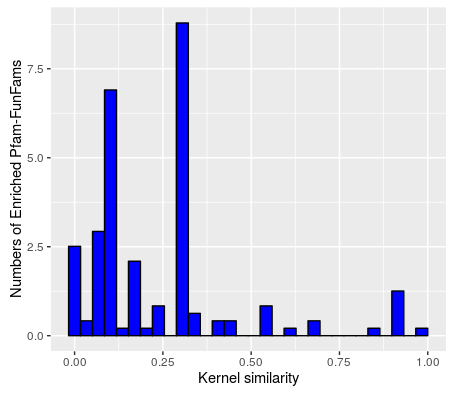
\includegraphics[width=.8\linewidth]{figures/ksim_plot.png}
	\centering
	\caption{Distribution of the kernel similarity measure across the Pfam-FunFam.}
	\label{ksim_plot}
\end{figure}
The results indicate that most of the Pfam-FunFam relatives are scattered across the functional protein network with majority of the Pfam-FunFam family having a similarity score lower than 0.5. This may explain one of the reason for the side effects associated with protein kinase inhibitors as their targets arequite diverse and could affect many biological pathways i.e. elicits multiple pharmacological responses in a given organism.\\
We then compared the kernel similarity of targeted kinase, all human kinases and the all the human proteins in the protein functional network. 
\begin{figure}[H]
	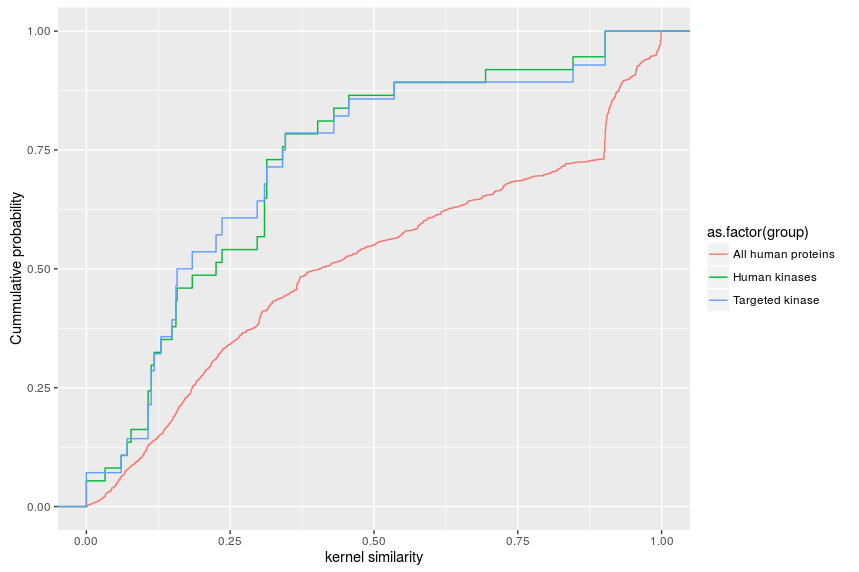
\includegraphics[width=\linewidth]{figures/ksim_hum.png}
	\centering
	\caption{Cummulative probability plot of the kernel similarity of all human targets compared against PKI-targets}
	\label{sim_plot}
\end{figure}
We observed as shown in figure \ref{sim_plot} that the targeted kinases has a lower kernel similarity as compared to the distribution of the kernel similarity of the all human proteins in the network however, there is no difference between the targetd kinases and all the human kinases as they show the same distribution as observed in the figure \ref{sim_plot}. To furthermore corroborate  our observation, we used another modular measure called DS$\_$score which was reported by \cite{menche2015uncovering}. The DS$\_$score measures the network distance of proteins  belonging to a group of drug-targets and compares their closeness to random expectation. We observed that there is a significant difference between DS$\_$score of the target proteins compared to random ($P$ $\le$ $1.116\times10^{-8}$, $Mann-Whitney$ \text{U-test}). The lower the DS$\_$score, the more aggregated the proteins in a network. This observation hence shows that the targeted kinases are quite clustered in a protein functional network compared to random proteins. 
\begin{figure}[H]
	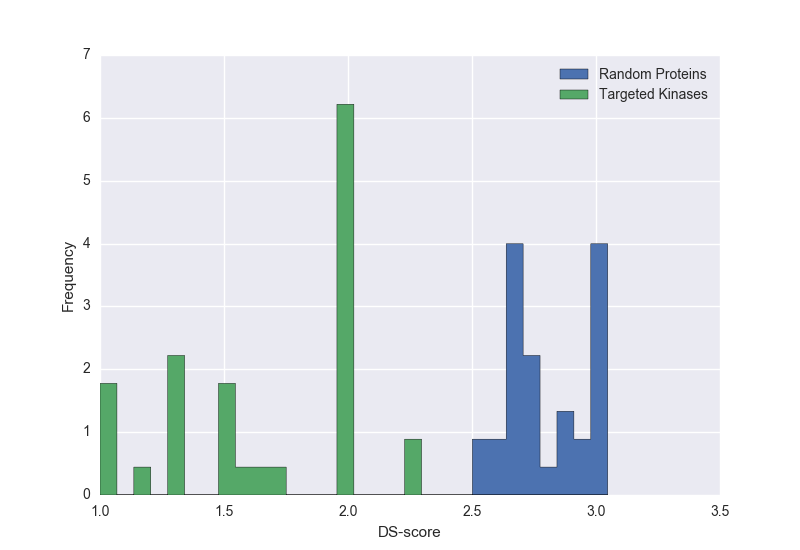
\includegraphics[width=.9\linewidth]{figures/mean_ds.png}
	\centering
	\caption{Distribution plot of the DS-measure of PKI-targets  compared against random proteins in a protein functional network}
	\label{ds_plot}
\end{figure}

\subsection*{Structural coherence of the binding site of the enriched Pfam-FunFam relatives}
The work published by \cite{elkins2016comprehensive} reported some of the solved structures of the binding of inhibitors from the PKIS with some kinases. The crystal structures of the inhibitor (CHEMBL237571) with the lymphocyte-oriented kinase (LOK) in the inactive DFG-out state (PDB-ID:4USD) and active DFG-in state (PDB-ID: 4USE) have been deposited in PDB. Therefore, using this example, we were interested in observing the binding site conservation across members of the Pfam-FunFam this target belongs to.\\
The target for this inhibitor belongs to the Pfam-FunFam PF00069.62355 (a STE-group kinase) that has about 80 relatives. Using the SIFTS mapping of UniProt-sequences to PDB structures, we were able to identify 15 members (about 18\%) of this family with PDB structures. In case of multiple structures of the same kinase, firstly, we find the structure without ligands, otherwise we chose the best resolved structure for the particular kinase.\\

\begin{table}[H]
\centering
\caption{The list of Pfam-FunFam (PF00069.62355) relatives with structural information}
\label{pfam-62355}
\begin{tabular}{|l|l|l|}
\hline
UniProt-ID & PDB-ID & Resolution (Å) \\ \hline
O95819     & 4u3y   & 1.45           \\ \hline
Q9P289     & 3ggf   & 2.35           \\ \hline
Q9P286     & 2f57   & 1.80           \\ \hline
O96013     & 2j0i   & 1.60           \\ \hline
Q8IVH8     & 5j5t   & 2.85           \\ \hline
Q9Y6E0     & 3a7f   & 1.55           \\ \hline
Q13153     & 1yhv   & 1.80           \\ \hline
Q9UKE5     & 2x7f   & 2.80           \\ \hline
Q9H2G2     & 2j51   & 2.10           \\ \hline
Q9NQU5     & 2c30   & 1.60           \\ \hline
Q99759     & 2o2v   & 1.83           \\ \hline
Q9Y2U5     & 5ex0   & 2.70           \\ \hline
Q13177     & 3pcs   & 2.86           \\ \hline
O00506     & 2xik   & 1.97           \\ \hline
O94804     & 2j7t   & 2.00           \\ \hline
\end{tabular}
\end{table}
We structurally superposed the members of this family to give a pictorial representataion of the conservation of the relatives and binding residues interacting with the CHEMBL237571. This family was found to be structurally coherent as the SSAP score gave an RMSD of $1.11 \pm 0.48$. 
\begin{figure}[H]
	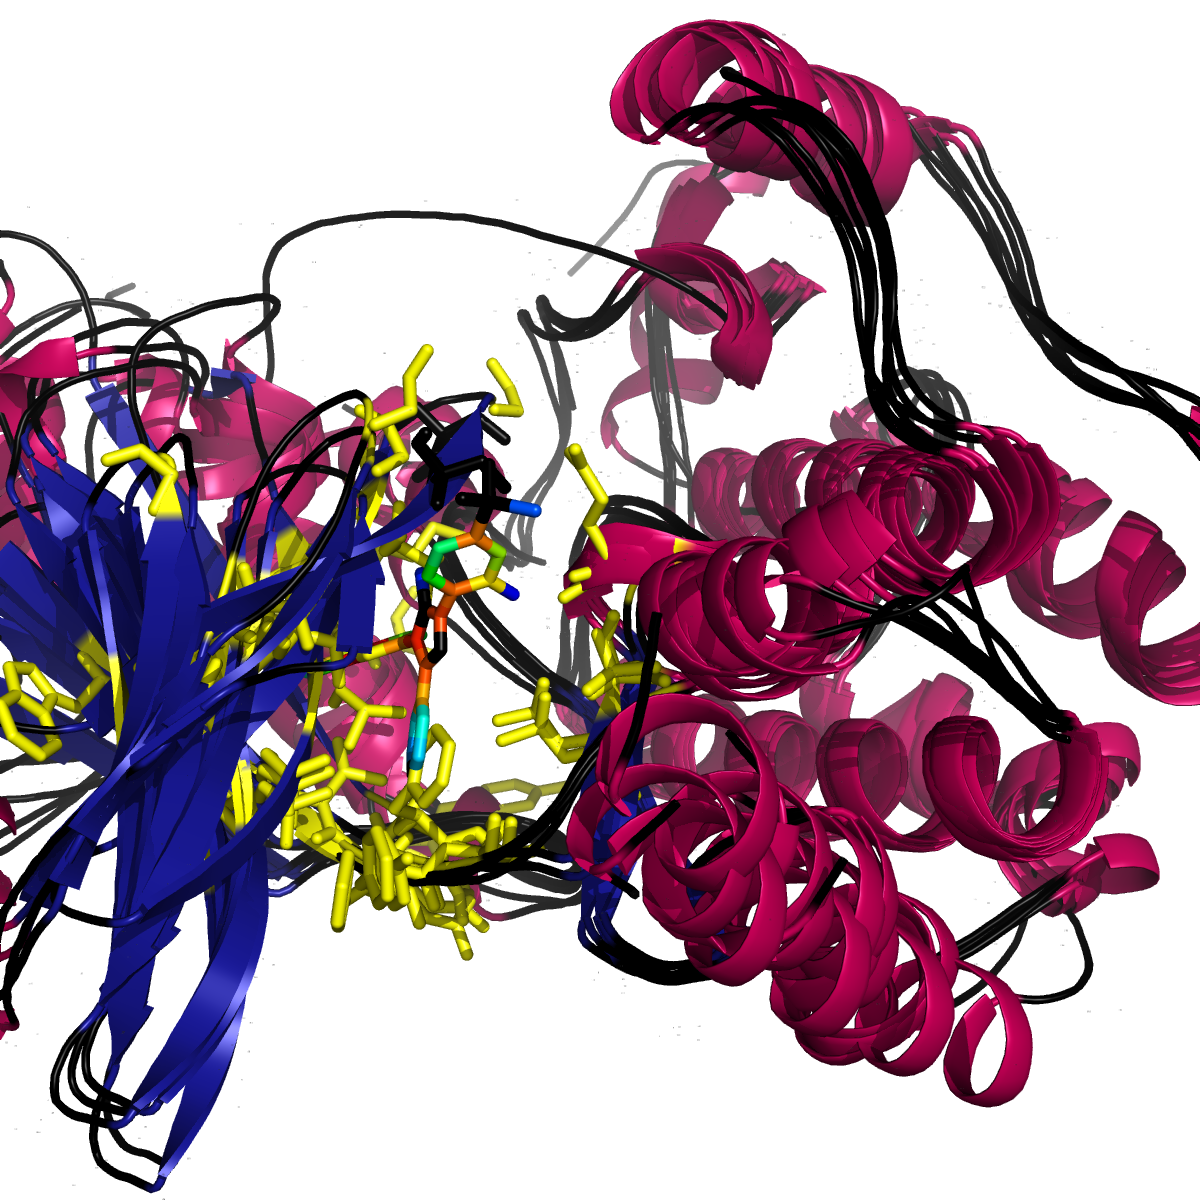
\includegraphics[width=.8\linewidth]{figures/superpose_4use.png}
	\centering
	\caption{Structural alignment and superposition of the relatives in Pfam-FunFam based on the alignment of the binding region. The interacting residues are coloured in yellow while the secondary structures are coloured accordingly (Beta sheet(blue), alpha (Magenta), the inhibitor is coloured in rainbow.}
	\label{struct_align}
\end{figure}
\subsection*{Network analysis of MutFams enriched with kinases}
We considered the network properties of mutation families (MutFams) which are enriched domain families that are highly mutated in a disease condition (cancer in this case) and compare the outcome with human variation data (HumVar). This approach was taken to study the kinases involved in diseases and examine the network properties of these mutation families in comparison with the targeted kinase FunFams.
\begin{figure}[H]
	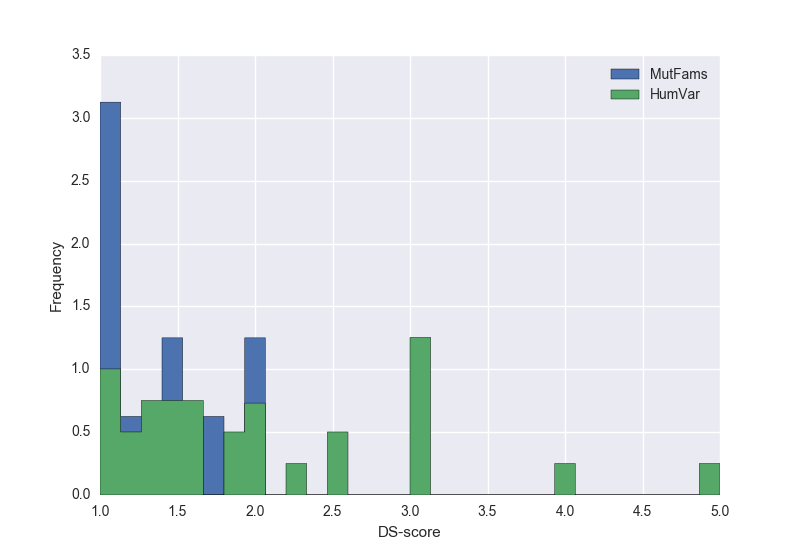
\includegraphics[width=\linewidth]{figures/mutvar.png}
	\centering
	\caption{DS-measure of the MutFam in comparison with the HUMVAR}
	\label{mutvar}
\end{figure}
Figure \ref{mutvar} shows a plot of the distribution of the DS-score between MutFams and HumVar. There is a significant difference between these two sets of genes as the MutFams are highly clustered in the human functional network as compared to the HumVar ($P=$ $0.00645$). \\
This indicate that the relatives of the MutFams are closely associated in the protein network and the MutFams therefore provides a reasonable annotation of disease genes with lower side effects anticipated when these families are targeted in a diseased condition.
\begin{figure}[H]
	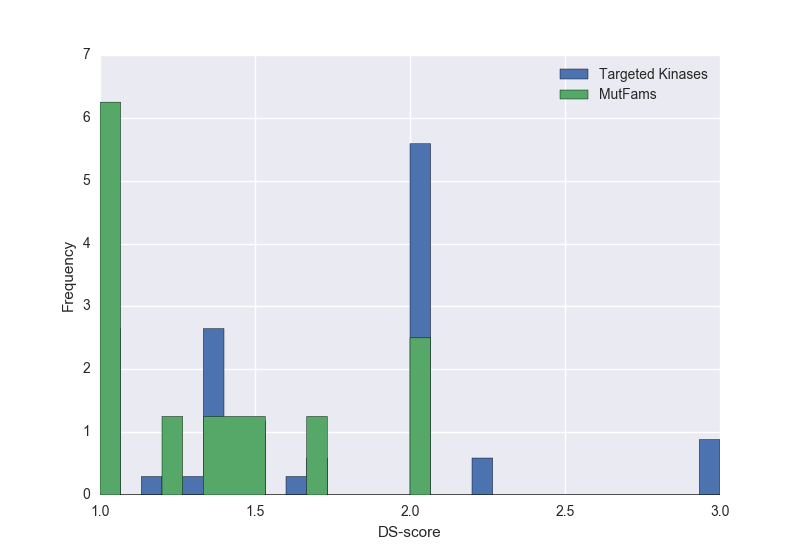
\includegraphics[width=\linewidth]{figures/muttarg.png}
	\centering
	\caption{DS-measure of the MutFam in comparison with the targeted kinases}
	\label{muttarg}
\end{figure}
The DS-score of the MutFams were compared with the targeted kinases (figure \ref{muttarg}), these different sets of genes tend to be clustered in the same fashion as there is no difference in the observed DS-score of the MutFams and the targeted kinases ($P=$ $0.0191$). This indicate that the targeted kinases shares similar network characteristics as the mutated sets of genes that are implicated in human diseases. These MutFams are potential therapeutic targets that could be harnessed and considered for therapeutic purposes.

\begin{table}[!htbp]
\fontsize{9}{10}\selectfont
\centering
\caption{The mutfam classes and their representation in Pfam-FunFams with the  similarity measure in the protein functional network}
\label{mutfam-table}
\begin{tabular}{|l|l|l|l|l|l|l|}
\hline
Cancer Types & CATH-FunFam          & Pfam-FunFam     & \%overlap & No of Drugs & Kernel-sim & DS-score \\ \hline
LGG          & 1.10.510.10.FF78531  & PF07714.FF13154 & 47.1      & 2           & 0.846             & 1.2      \\ \hline
LGG          & 1.10.510.10.FF79008  & PF00069.FF27817 & 46.2      &             & 0.541267          & 1        \\ \hline
BLCA         & 1.25.40.70.FF2223    & PF00454.FF1812  & 43.2      &             & 0.662619          & 1.5      \\ \hline
BRCA         & 3.30.200.20.FF2866   &                 &           &             &                   &          \\ \hline
BRCA         & 2.30.29.30.FF22238   & PF00069.FF25168 & 14.2      & 4           & 0.319             & 1        \\ \hline
BRCA         & 1.10.1070.11.FF1687  & PF00454.FF1812  & 37.3      &             & 0.662619          & 1.5      \\ \hline
BRCA         & 1.25.40.70.FF2223    & PF00454.FF1812  & 43.2      &             & 0.662619          & 1.5      \\ \hline
COAD         & 3.30.200.20.FF64824  &                 &           &             &                   &          \\ \hline
COAD         & 1.20.120.330.FF23932 &                 &           &             &                   &          \\ \hline
COAD         & 1.10.510.10.FF78531  & PF07714.FF13154 & 47.1      & 2           & 0.846             & 1.2      \\ \hline
COAD         & 1.10.1070.11.FF1687  & PF00454.FF1812  & 37.3      &             & 0.662619          & 1.5      \\ \hline
COAD         & 1.10.510.10.FF79298  & PF00069.FF62569 & 100       &             & 0.584709          & 1        \\ \hline
COAD         & 1.25.40.70.FF2223    & PF00454.FF1812  & 43.2      &             & 0.662619          & 1.5      \\ \hline
COAD         & 1.10.510.10.FF78966  & PF07714.FF3369  & 35.7      & 1           & 0.097             &          \\ \hline
COAD         & 1.10.510.10.FF79140  & PF07714.FF13122 & 100       &             & 0.220333          & 1        \\ \hline
GBM          & 1.10.510.10.FF79478  & PF00069.FF61939 & 45.5      &             & 0.694             & 1        \\ \hline
GBM          & 3.30.505.10.FF4305   &                 &           &             & 0.509667          &          \\ \hline
GBM          & 1.10.510.10.FF79008  & PF00069.FF27817 & 46.2      &             & 0.541267          & 1        \\ \hline
GLI          & 1.10.510.10.FF78531  & PF07714.FF13154 & 47.1      & 2           & 0.846             & 1.2      \\ \hline
GLI          & 1.10.510.10.FF79478  & PF00069.FF61939 & 45.5      &             & 0.694             & 1        \\ \hline
GLI          & 1.10.510.10.FF79008  & PF00069.FF27817 & 46.2      &             & 0.509667          & 1        \\ \hline
GLI          & 3.30.505.10.FF4305   &                 &           &             &                   &          \\ \hline
GLI          & 1.25.40.70.FF2223    & PF00454.FF1812  & 43.2      &             & 0.662619          & 1.5      \\ \hline
KIRC         & 1.25.40.70.FF2223    & PF00454.FF1812  & 43.2      &             & 0.662619          & 1.5      \\ \hline
LAML         & 1.10.510.10.FF78745  & PF07714.FF13026 & 53.1      & 17          & 0.184             & 1.2      \\ \hline
LIHC         & 1.25.40.70.FF2223    & PF00454.FF1812  & 43.2      &             & 0.662619          & 1.5      \\ \hline
LIHC         & 3.30.60.20.FF5564    & PF00069.FF62318 & 23.9      & 6           & 0.3411            & 1.17     \\ \hline
LUAD         & 3.30.200.20.FF1240   &                 &           &             &                   &          \\ \hline
LUAD         & 3.30.200.20.FF64824  &                 &           &             &                   &          \\ \hline
LUAD         & 1.10.510.10.FF79008  & PF00069.FF27817 & 46.2      &             & 0.541267          & 1        \\ \hline
LUAD         & 1.10.510.10.FF79228  & PF00069.FF62599 & 71.4      &             & 0.588333          & 1.5      \\ \hline
LUSC         & 1.25.40.70.FF2223    & PF00454.FF1812  & 43.2      &             & 0.662619          & 1.5      \\ \hline
PAAD         & 1.10.510.10.FF78763  & PF00069.FF62351 & 43.5      & 1           & 0.155692          & 1.5      \\ \hline
READ         & 1.10.510.10.FF78531  & PF07714.FF13154 & 47.1      &             & 0.846             & 1.2      \\ \hline
READ         & 1.10.1070.11.FF1687  & PF00454.FF1812  & 37.3      &             & 0.662619          & 1.5      \\ \hline
READ         & 1.10.510.10.FF78946  & PF00069.FF62345 & 43.8      & 5           & 0.4562            & 1.72     \\ \hline
SKCM         & 1.10.510.10.FF78531  & PF07714.FF13154 & 47.1      & 2           & 0.846             & 1.2      \\ \hline
THCA         & 1.10.510.10.FF78531  & PF07714.FF13154 & 47.1      & 2           & 0.846             & 1.2      \\ \hline
UCEC         & 1.25.40.70.FF2223    & PF00454.FF1812  & 43.2      &             & 0.662619          & 1.5      \\ \hline
\end{tabular}
\end{table}


\newpage
\bibliography{kin_references.bib}
\bibliographystyle{apa}
%\printbibliography
\end{document}
